\documentclass[12pt]{report}
\usepackage[english]{babel}
\usepackage{xcolor}
\usepackage{amsmath}
\usepackage{amssymb}
\usepackage{amsfonts}
\usepackage{empheq}
\usepackage{bbold}
\usepackage{cancel}
%\usepackage[authoryear,round,longnamesfirst]{cite}
\usepackage{natbib}
\usepackage[nottoc]{tocbibind}
\usepackage{url}
\usepackage[dvips,letterpaper,margin=1in,bottom=1in]{geometry}
\usepackage{hyperref}
\usepackage{mathrsfs}
\usepackage{enumerate}
\usepackage{amscd}
\usepackage{dirtree}
\usepackage[all,cmtip]{xy}
%\usepackage{bbm}
\usepackage[utf8]{inputenc}
%\usepackage[left=2.5cm,right=2.5cm,top=3cm,bottom=3.5cm]{geometry}

% JOURNAL NAMES:
\newcommand{\aap}{Astron. Astrophys.}
\newcommand{\apj}{Ap. J.}
\newcommand{\apjl}{Astrophys. J. Lett.}
\newcommand{\ssr}{Space Science Reviews}
\newcommand{\nphysa}{Nucl. Phys. A}
\newcommand{\arnps}{Annu. Rev. Nucl. \& Part. Sci.}
\newcommand{\araa}{Annu. Rev. Astron. \& Astrophys.}
\newcommand{\physrep}{Phys. Rep.}
\newcommand{\prd}{Phys. Rev. D.}
\newcommand{\prl}{Phys. Rev. Lett.}
\newcommand{\pr}{Phys. Rev.}
\newcommand{\mnras}{Monthly Not. Royal Astron. Soc.}
\newcommand{\nat}{Nature}
\newcommand{\apss}{Astrophysics and Space Science}


\newcommand\red[1]{\textcolor{red}{#1}}
\newcommand\blue[1]{\textcolor{blue}{#1}}
\newcommand\green[1]{\textcolor{green}{#1}}
\newcommand\teal[1]{\textcolor{teal}{#1}}


\newcommand*{\titleGM}{\begingroup % Create the command for including the title page in the document
	\hbox{ % Horizontal box
		\hspace*{0.2\textwidth} % Whitespace to the left of the title page
		\rule{1pt}{\textheight} % Vertical line
		\hspace*{0.05\textwidth} % Whitespace between the vertical line and title page text
		\parbox[b]{0.75\textwidth}{ % Paragraph box which restricts text to less than the width of the page
			{\noindent\Huge\bfseries TOV Equations\\}\\[2\baselineskip] % Title
			% Tagline or further description
			{\large \textsc{ OMAR ELÍAS VELASCO CASTILLO }} % Author name
			
			\vspace{0.5\textheight} % Whitespace between the title block and the publisher
			{\noindent Universidad Nacional Autónoma de México \\ Instituto de Astronomía, Ciudad Universitaria }\\[\baselineskip] % Publisher and logo
	}}
	\endgroup}
% Sets margins and page size
\pagestyle{empty} % Removes page numbers
\makeatletter % Need for anything that contains an @ command 
\renewcommand{\maketitle} % Redefine maketitle to conserve space
{ \begingroup \vskip 10pt \begin{center} \Huge {\bf \@title}
		\vskip 10pt \large \@author \hskip 20pt \@date \end{center}
	\vskip 10pt \endgroup \setcounter{footnote}{0} }
\makeatother % End of region containing @ commands

% ***********************************************************
% ********************** END HEADER *************************
% ***********************************************************




\begin{document}
	\titleGM
	
	
	
	\chapter{Introduction}
	%
	\chapter{Fundamentals of Hydrodynamics and Ideal Fluids}
	%
	Thermodynamics (hydrodynamics) is the branch of physics that helps us study gases (fluids) in physical systems with certain fundamental state variables and their relationship with the boundaries and surroundings of the system in which they are found. Both disciplines are equivalent in their treatment and possess laws that regulate and describe in detail how these system variables behave at macroscopic scales and, in turn, relate to the microphysics of the most elementary components of the gas or fluid.\\
	
	The most important law for the purposes of this work is the first law, which is typically stated with the following equation:
	%
	\begin{equation}
		dU = \delta Q-\delta W.
	\end{equation}
	%
	The thermodynamic variable associated with the internal energy of the system $U$ has a total exact differential $dU$ which, in any thermodynamic equilibrium process, results from the difference between the inexact differentials of heat exchange $\delta Q$ and the work performed by the system with its boundaries and surroundings $\delta W$. In classical mechanics, it is recalled that the differential of work done by an object along a path $d\vec{r}$ is:
	%
	\begin{equation}
		\delta W=\vec{F}\cdot d\vec{r}.
	\end{equation}
	%
	This work performed by an object is path-dependent for the displacement along a certain trajectory given by $d\vec{r}$ and, therefore, it is an inexact differential. In a generalized case, we can assume that both $\vec{F}$ and $d\vec{r}$ are projected in the same direction (or we reorient them to do so) and define a generalized work performed by the system as:
	%
	\begin{equation}
		\delta W = A\,da,
	\end{equation}
	%
	where $A$ is a generalized force and $a$ is a generalized displacement.\\
	
	For example, in systems such as gases and fluids, the pressure $P$ exerted by normal stresses in the medium where an element of our substance is found will be our generalized force, while the volume $V$ will be our generalized displacement. Moreover, by the thermodynamic definition of entropy in reversible equilibrium processes,
	%
	\begin{equation}
		\delta Q=TdS,
	\end{equation}
	%
	for these systems it is very common to find that the first law is rewritten as:
	%
	\begin{align}
		dU = TdS-PdV+\mu dN.
	\end{align}
	%
	\section{Polytropic Process}
	A thermodynamic (hydrodynamic) process in our system is called a polytropic process if it satisfies the relation:
	%
	\begin{equation}
		\delta Q=  C \,dT\qquad \text{with }C\in(-\infty,\infty).
	\end{equation}
	%
	Some typical examples of these are:
	%
	\begin{itemize}
		\item An adiabatic process, for which $C=0$.
		\item An isothermal process, for which $C\to\infty$.
	\end{itemize}
	%
	We say that our system is in local thermodynamic (hydrodynamic) equilibrium when the mean free path of the particles that make up the gas or fluid is much smaller than the characteristic scales of the system (such as, for example, the distances from the particles to the boundaries that delimit it). This condition allows us to assign a relation depending on the fundamental variables of the system’s internal state to describe it macroscopically: an equation of state. This is a function of the following state variables: generalized force, rest-mass density $\rho$, specific entropy $s$, and chemical potential $\mu$,
	%
	\begin{equation}
		f(A,\rho,s,\mu)=0.
	\end{equation}
	%
	In the typical case of a gas or fluid in thermodynamics or hydrodynamics, this allows us to rewrite an equation of state (abbreviated EoS) as the relation:
	%
	\begin{equation}
		P=P(\rho,s,\mu).
	\end{equation}
	%
	As an example to mention, there is an equation of state for a polytropic process as it will be shown below, of the form: $P=K\rho^\gamma$. Alternatively, it is very useful to define more thermodynamic variables that help us describe the system. We have the following \red{Table \ref{tab:vars}} to assist in this regard.
	%
	\begin{table}[]
		\centering
		\resizebox{\textwidth}{!}{%
			\begin{tabular}{|l|l|l|}
				\hline
				Variable & Symbol &  Fundamental Expression   \\ \hline
				Rest mass & $m_0$ &    \\
				Volume & $V$ & \\
				Number of particles & $N$ & \\
				Number of baryons & $N_b$ & \\
				Number of moles & $\eta$ & Widely used for ideal gas ($PV=\eta RT$)\\
				& & \\
				Specific entropy & $s$ & $\dfrac{S}{m_0N}$ \\
				& & \\
				Number density & $n$ & $\dfrac{N}{V}$   \\
				& & \\
				Baryon number density & $n_b$ & $\dfrac{N_b}{V}$ \\
				Rest-mass density & $\rho$ & $m_0n = \dfrac{m_0N}{V};\qquad m_0n_b = \dfrac{m_0N_b}{V}$ \\
				& & \\
				Specific internal energy & $\epsilon$ & $d\epsilon=\dfrac{dU}{m_0N}=Tds - Pd\left(\dfrac{1} {\rho}\right)+\dfrac{\mu}{m_0 N} dN$ \\
				& & \\
				Total energy density & $e$ & $\rho(c^2+\epsilon)$ \\
				& & \\
				Enthalpy density & $w$ & $e+P=\rho(c^2+\epsilon)+P$\\
				& & \\
				Specific enthalpy & $h$ & $\dfrac{H}{m_0 N}=\dfrac{w}{\rho}=c^2+\epsilon+\dfrac{P}{\rho}$ \\
				& & \\
				\hline
			\end{tabular}
			%
		}
		\caption{\small Scheme showing the different state variables typically found in thermodynamic (hydrodynamic) processes and their fundamental relations, which will be very useful in this work.}
		\label{tab:vars}
	\end{table}
	%
	\section{Ideal gas}
	An ideal gas or fluid (also called a perfect gas or fluid) is defined as a fluid for which there is no diffusion or heat transfer across its boundaries to its surroundings and that also presents no viscosity. In classical thermodynamics, it is found that in such a substance, the internal energy depends only on the absolute temperature of the system and obeys the following EoS:
	%
	\begin{equation}
		PV = \eta RT = Nk_\text{B}T 
	\end{equation}
	%
	Here without loss of generality, the next calculations will be performed for a certain $n$ number density, regarding a density for a number $N^*$ of moles, particles or baryons. Let the ideal gas equation be:
	%
	\begin{equation}
		P= nKT \label{eq:idealgas}
	\end{equation}
	%
	where $k$ is the adequate constant of proportionality depending on the density employed (universal constant for ideal gases, Boltzmann's constant). Then, the rest-mass density and the number density are each defined as:
	\begin{align}
		\rho &= \frac{m_0N^*}{V} = m_0n\\
		n&= \frac{N^*}{V} 
	\end{align}
	%
	If we use $T$ and ``$a$'' as fundamental variables of $U$, we have:
	
	\begin{equation}
		dU = \left(\frac{\partial U}{\partial T}\right)_a dT + \left(\frac{\partial U}{\partial a}\right)_T da
	\end{equation}
	%
	Substituting into the First Law:
	\begin{align}
		\delta Q &= dU + A(T,a)da \\
		\Rightarrow\;\delta Q &= \left(\frac{\partial U}{\partial T}\right)_a dT + \left[A(T,a) + \left(\frac{\partial U}{\partial a}\right)_T\right]da\\
		\Rightarrow\;C &= \frac{\delta Q}{dT} = \left(\frac{\partial U}{\partial T}\right)_a + \left[A(T,a) + \left(\frac{\partial U}{\partial a}\right)_T\right]\frac{da}{dT}
	\end{align}
	%
	where, in the last step, we use the thermodynamic definition of heat capacity:
	%
	\begin{equation}
		C = \dfrac{\delta Q}{dT}.
	\end{equation}
	%
	Now, for this quantity we can have two different cases:
	\begin{align*}
		\begin{cases}
			a = \text{constant} \\
			A = \text{constant}
		\end{cases}
	\end{align*}
	%
	\begin{enumerate}
		\item If $a = \text{const} \Rightarrow da=0$
		%
		\begin{align}
			\Rightarrow C_a=\left(\dfrac{\delta Q}{dT}\right)_a = \left(\dfrac{\partial U}{\partial T}\right)_a.
		\end{align}
		%
		\item If $A = \text{const} \Rightarrow dA = 0$
		%
		\begin{align}
			\Rightarrow C_A = \left(\frac{\delta Q}{d T}\right)_A = C_a + \left[A + \left(\frac{\partial U}{\partial a}\right)_T\right]\left(\frac{\partial a}{\partial T}\right)_A
		\end{align}
		%
		because:
		\begin{align}
			\left(\frac{d a}{d T}\right)_A = \left(\frac{\partial a}{\partial T}\right)_A + \frac{\partial a}{\partial A}\left(\frac{\partial A}{\partial T}\right)_A = \left(\frac{\partial a}{\partial T}\right)_A
		\end{align}
		
		\begin{align}
			\Rightarrow \boxed{C_A - C_a = \left[A + \left(\frac{\partial U}{\partial a}\right)_T\right]\left(\frac{\partial a}{\partial T}\right)_A } 
		\end{align}
	\end{enumerate}
	%
	Then,
	%
	\begin{align}
		\delta Q &= C\,dT = C_a\,dT + \left[A + \left(\frac{\partial U}{\partial a}\right)_T\right]da \\
		\Rightarrow &(C - C_a)\,dT = \left[A + \left(\frac{\partial U}{\partial a}\right)_T\right]da
	\end{align}
	%
	But, from the above:
	%
	\begin{align}
		\left[A + \left(\frac{\partial U}{\partial a}\right)_T\right] = (C_A - C_a)\left(\frac{\partial T}{\partial a}\right)_A \\
		\therefore \boxed{(C - C_a)\,dT = (C_A - C_a)\left(\frac{\partial T}{\partial a}\right)_Ada }
	\end{align}
	%
	That is:
	\begin{equation}
		dT + \frac{C_A-C_a}{C_a-C}\left(\frac{\partial T}{\partial a}\right)_A da = 0 
	\end{equation}
	where $C_a-C = -(C-C_a)$.\\
	
	Then, since:
	%
	\begin{align}
		dT &= \left(\frac{\partial T}{\partial A}\right)_a dA + \left(\frac{\partial T}{\partial a}\right)_A da  \\
		\Rightarrow &\left(\frac{\partial T}{\partial A}\right)_a dA + \left(\frac{\partial T}{\partial a}\right)_A da + \frac{C_A-C_a}{C_a-C}\left(\frac{\partial T}{\partial a}\right)_A da = 0\nonumber\\
		\Rightarrow &\left(\frac{\partial T}{\partial A}\right)_a dA + \frac{C_a-C+C_A-C_a}{C_a-C}\left(\frac{\partial T}{\partial a}\right)_A da = 0 \nonumber\\
		\Rightarrow &\left(\frac{\partial T}{\partial A}\right)_a dA + \frac{C_A-C}{C_a-C}\left(\frac{\partial T}{\partial a}\right)_A da = 0
	\end{align}
	
	For an ideal gas: $A \rightarrow P$, $a \rightarrow V$ 
	\begin{equation}
		\Rightarrow \left(\frac{\partial T}{\partial P}\right)_V dP + \frac{C_P-C}{C_V-C}\left(\frac{\partial T}{\partial V}\right)_P dV = 0 
	\end{equation} 
	%
	Define the number:
	%
	\begin{equation}
		\gamma = \frac{C_P-C}{C_V-C},
	\end{equation}
	%
	as a polytropic index (note: this is not the same as the adiabatic index, as we will see below).\\
	
	And since $P= nkT$, see \textcolor{red}{Eq. \ref{eq:idealgas}}:
	\begin{align}
		T &= \frac{P}{nk} =\frac{PV}{N^*k}\Rightarrow \boxed{\left(\frac{\partial T}{\partial P}\right)_V = \frac{V}{N^*k}, \quad
			\left(\frac{\partial T}{\partial V}\right)_P = \frac{P}{N^* k}} \\
		\Rightarrow &\;\frac{V}{N^*k}dP + \gamma\frac{P}{N^*k}dV = 0 \\
		\Rightarrow &\;\frac{dP}{P} = -\gamma\frac{dV}{V}\\
		\Rightarrow &\;\ln P = -\gamma\ln V + C_1 =-\ln V^\gamma + C_1 \\
		\Rightarrow &\; \boxed{PV^\gamma = C_1 = \text{constant}} \label{eq:prelpoly}
	\end{align} 
	%
	This last relation is the classical definition of a polytropic process in the form of an EoS, showing then how the ideal gas is a particular case of a polytropic process. In other words, we just found that an ideal gas implies a determined case of a polytropic one. 
	%
	\section{Adiabatic Process and Equation of State}
	%
	An adiabatic process is a very particular class of polytropic process and is one for which $C=0$. Therefore, in an adiabatic process we have:
	%
	\begin{equation}
		\gamma = \dfrac{C_P-C}{C_V-C} = \dfrac{C_P}{C_V} = \Gamma
	\end{equation}
	%
	Transforming the \red{Eq. \ref{eq:prelpoly}} above, since $ V = \frac{N^*}{n} = \frac{m_0N^*}{\rho}$:
	\begin{align}
		P\left(\frac{m_0N^*}{\rho}\right)^{\Gamma} &= \text{constant} = C_1 \\
		P &= \frac{C_1}{(m_0N^*)^{\Gamma}} \rho^{\;\Gamma}= K\rho^{\;\Gamma}
	\end{align}
	%
	Defining for an adiabatic process: 
	%
	\begin{equation}
		\Gamma = \gamma = 1 + \frac{1}{n_f}
	\end{equation}
	%
	as a corresponding polytropic index, we are left with the following EoS:
	\begin{equation}
		P = K\rho^{\;\Gamma} \label{eq:adiabpolyeos}
	\end{equation}
	%
	Note: \red{Eq. \ref{eq:prelpoly}} is the generic EoS for a polytropic process, whereas \red{Eq. \ref{eq:adiabpolyeos}} is the form of that EoS for an adiabatic process, and its corresponding adiabatic index. In general, a polytropic index can have various possible values, as $\gamma \in (-\infty,+\infty)$ is not bounded. The adiabatic index $\Gamma$ will depend on the specific adiabatic process or EoS taken into account.\\
	
	Is there though a form for writing an EoS for an ideal gas following an adiabatic process? In the developments below, we will take the specific internal energy as: $\frac{U}{m_0N^*} = \epsilon$.\\
	
	From the first law of thermodynamics,
	\begin{align}
		d\epsilon &= Tds - Pd\left(\frac{1}{\rho}\right) = Tds + \frac{P}{\rho^2}d\rho\\
		\Rightarrow &\;C_V = \left(\frac{\partial U}{\partial T}\right)_V= m_0 N^*\left(\frac{\partial \epsilon}{\partial T}\right)_V.
	\end{align} 
	
	For an ideal gas, a well-known result in thermodynamics is that its total internal energy depends only on its temperature: $U = U(T)$.  Then:
	
	\begin{align}
		\Gamma &= \frac{C_P}{C_V} \\
		\Gamma-1 &= \frac{C_P-C_V}{C_V} = \frac{nk}{C_V} \\
		\Rightarrow &\; C_V = \frac{nk}{\Gamma-1}
	\end{align}
	
	So finally, $dU=U'(T)dT=\left(\frac{\partial U}{\partial T}\right)_VdT$
	\begin{equation}
		\Rightarrow U =  \epsilon \, m_0 N^* = C_VT = \frac{nkT}{\Gamma-1} = \frac{PV}{\Gamma-1}=\frac{Pm_0N^*}{\rho(\Gamma-1)} 
	\end{equation}
	
	\begin{equation}
		\therefore \boxed{P = \rho \epsilon(\Gamma-1).\;}\label{eq:adiab}
	\end{equation}
	%
	The last EoS is known as an adiabatic EoS, or also as a Gamma-law EoS. In the latest developments, the polytropic index is now $\Gamma$, as is usual when dealing with the ideal gas equation for an adiabatic fluid. With this result, we have just shown that for an adiabatic process, this new EoS is equivalent to the ideal gas equation.\\
	
	Finally, it is worthy to include here a last result which is very important, as it is shown in the literature. From the last derivations, a familiarity between the EoS for a polytrope and an adiabatic process seems to arise. Both polytropic and adiabatic gas are indeed related to the ideal gas. However, it is important to stress that what we have seen up to here only confirms that the ideal gas is a particular case of a polytropic process, and that the ideal gas, when adiabatic, finds a new form for its EoS.\\
	
	Is there a scenario where an adiabatic EoS (gas) can be represented and equivalent to a polytropic one? The answer is yes, and before getting hands down on to it, there is a subtlety that needs to be mentioned before: the polytropic EoS in the form $P=K\rho^\gamma$ only depends in the rest-mass density (it is barotropic), but the adiabatic EoS \red{\ref{eq:adiab}} is dependent in both the rest-mass density and the internal energy $\epsilon$. So if there was an equivalence between both equations of state, there should be a way to not violate this extra dependency in the internal energy.\\
	
	When a process is isentropic, that is, when it has constant entropy, the adiabatic process can be equivalent to that of a polytropic. Indeed, for a fluid that satisfies the ideal EoS and is also isentropic, the first law of thermodynamics can be written as:
	\begin{equation}
		d\epsilon= P\dfrac{dV}{m_0N} =\frac{P}{\rho^2}d\rho, 
	\end{equation} 
	
	because there $ds = 0$. If we consider that our ideal, isentropic gas follows a polytropic EoS, then:
	%
	\begin{align} 
		\Rightarrow &\;\epsilon = \int \frac{K\rho^\gamma}{\rho^2}d\rho = \frac{K\rho^{\gamma-1}}{\gamma-1} = \frac{P}{\rho(\gamma-1)}
	\end{align}
	%
	which therefore implies that for a polytropic EoS, we recover the Gamma-law EoS if and only if we prescribe an ideal gas with the extra ansatz $ds=0$. This is why in the literature, it is common to find that the adiabatic index is defined as:
	%
	\begin{equation}
		\boxed{\Gamma = \left(\frac{\partial \ln P}{\partial \ln \rho}\right)_s.\;}
	\end{equation}
	%
	As commented above, an adiabatic process respects $C=0$ and from there we could define an adiabatic index in a polytrope. Note that $ds=0$ is a particular case of this, that is, $\delta Q=0$, and which also agrees with $C=0$. Finally, an adiabatic process happens to be also an ideal one, since it has no heat transference, and therefore is sensitive to the internal kinetic energy. The rest-mass density in an adiabatic process is intrinsically dependent of the kinetic energy, although not explicitly stated. This is why some authors model adiabatic processes with a power-law polytrope in the enthalpy or the total energy density, rather than in the rest-mass density.
	%
	\chapter{TOV Equations as a Solution for a Static and Stationary Spacetime in Spherical Symmetry}
	%
	In this section, we will introduce the TOV (Tolman-Oppenheimer-Volkoff) equations to study a solution for a static spacetime in spherical symmetry, with a matter-energy contribution given by a perfect fluid.\\
	
	The line element in this spacetime looks in a general case as:
	%
	\begin{equation}
		ds^2 = -\alpha^2(t,r)dt^2+X^2(t,r)\,dr^2+r^2d\theta^2+r^2\sin^2\theta\, d\phi^2.
	\end{equation}
	%
	Here we are using spherical coordinates $(r,\theta,\phi)$ in space and the coordinate time $t$ measured by a static observer.
	If we further require that our spacetime is stationary, to find the hydrostatic equilibrium solution for our perfect fluid, this metric adopts the final form:
	%
	\begin{equation}
		\boxed{ds^2=-\alpha^2(r)dt^2+X^2(r)\,dr^2+r^2d\theta^2+r^2\sin^2\theta\, d\phi^2}\;. \label{eq:metrictov}
	\end{equation}
	%
	The energy-momentum tensor for a perfect fluid has the following expression:
	%
	\begin{align}
		T^{\mu\nu}=\rho h\,u^\mu u^\nu+Pg^{\mu\nu} \\
		=(e+P)\,u^\mu u^\nu+Pg^{\mu\nu}
	\end{align}
	%
	where $h=c^2+\epsilon+\frac{P}{\rho}$ is the specific enthalpy.\\
	
	In a general case, the components of the 4-velocity of an Eulerian observer who is at rest in a fixed coordinate system, from which they observe the fluid moving with some velocity (recall that it moves in space along the radial coordinate $r$, due to spherical symmetry), have components:
	%
	\begin{equation}
		u^\mu = (u^t,u^r,0,0)^T = \left(\dfrac{W}{\alpha},Wv^r,0,0\right)^T.
	\end{equation}
	%
	This result follows from the fact that, for an Eulerian observer:
	%
	\begin{equation}
		d\tau = \alpha \,dt
	\end{equation}
	%
	And if this observer sees the fluid moving at a velocity $v^i$
	\begin{equation}
		u^t = \dfrac{dt}{d\tau} = \dfrac{W}{\alpha}
	\end{equation}
	%
	Suppose we are studying the fluid from an Eulerian and static coordinate system, i.e., we place our observer at rest with a coordinate system that remains static relative to the fluid. Then, the components of the 4-velocity for our observer will simply be:
	%
	\begin{equation}
		u^\mu = (u^t,0,0,0)^T = \left(\dfrac{1}{\alpha},0,0,0\right)^T.
	\end{equation}
	%
	Thus, the components of the energy-momentum tensor for our perfect fluid will be:
	%
	\begin{align}
		T^{tt}&=\rho h u^t u^t + P g^{tt}= \dfrac{1}{\alpha^2}(\rho h - P)=\dfrac{e}{\alpha^2},\\
		T^{rr}&=Pg^{rr}=\dfrac{P}{X^2},\\
		T^{\theta\theta}&=Pg^{\theta\theta}=\dfrac{P}{r^2}, \\
		T^{\phi\phi}&=Pg^{\phi\phi}=\dfrac{P}{r^2\sin^2\theta}.
	\end{align}
	%
	Or equivalently, with the indices lowered, from the normalization condition $u_\mu u^\mu=-1$, we have:
	%
	\begin{equation}
		u_\mu = (u_t,0,0,0) = \left(-\alpha,0,0,0\right)=n_{\mu}\;;
	\end{equation}
	%
	which is exactly the covariant normal 4-vector (remember, an Eulerian observer is also sometimes regarded as a normal observer). Therefore,
	%
	\begin{align}
		T_{tt}&=\rho h u_t u_t + P g_{tt}= \alpha^2(\rho h - P)=e\alpha^2,\\
		T_{rr}&=Pg_{rr}=PX^2,\\
		T_{\theta\theta}&=Pg_{\theta\theta}=Pr^2, \\
		T_{\phi\phi}&=Pg_{\phi\phi}=Pr^2\sin^2\theta.
	\end{align}
	%
	Recall that Einstein’s equations (without a cosmological constant) are written as:
	%
	\begin{equation}
		G_{\mu\nu} = R_{\mu\nu}-\dfrac{1}{2}g_{\mu\nu}R=8\pi T_{\mu\nu}.
	\end{equation}
	%
	Or equivalently,
	\begin{equation}
		R_{\mu\nu} = 8\pi(T_{\mu\nu} - \tfrac{1}{2}g_{\mu\nu}T).
	\end{equation}
	%
	From the definitions,
	\begin{equation}
		R_{\mu\nu} = R^{\sigma}_{\mu\sigma\nu} = \partial_{\sigma}\Gamma^{\sigma}_{\mu\nu} - \partial_{\nu}\Gamma^{\sigma}_{\sigma\mu} + \Gamma^{\sigma}_{\sigma\epsilon}\Gamma^{\epsilon}_{\mu\nu} - \Gamma^{\sigma}_{\nu\epsilon}\Gamma^{\epsilon}_{\sigma\mu}
	\end{equation}
	
	\begin{equation}R = g^{\mu\nu}R_{\mu\nu}\end{equation}
	
	\begin{align}
		\Rightarrow G_{\mu\nu} &= R_{\mu\nu} - \frac{1}{2}Rg_{\mu\nu} \\
		&=\delta^{\gamma}_{\mu}\delta^{\xi}_{\nu}R_{\gamma\xi} - \frac{1}{2}g_{\mu\nu}g^{\gamma\xi}R_{\gamma\xi}\\
		&= (\delta^{\gamma}_{\mu}\delta^{\xi}_{\nu} - \frac{1}{2}g_{\mu\nu}g^{\gamma\xi})R_{\gamma\xi}
	\end{align}
	%
	where $\delta_\alpha^\beta=g_{\alpha\lambda}g^{\lambda^\beta}$. Let's recall that:
	\begin{equation}g_{\mu\nu} = \text{diag}(-\alpha^2, X^2, r^2, r^2\sin^2\theta)\end{equation}
	
	and we know that:
	\begin{equation} d\text{s}^2 = g_{\mu\nu}dx^{\mu}dx^{\nu}\end{equation}
	
	\begin{equation}
		g^{\mu\nu} = \text{diag}\left(-\frac{1}{\alpha^2}, \frac{1}{X^2}, \frac{1}{r^2}, \frac{1}{r^2\sin^2\theta}\right)
	\end{equation}
	
	Where $T = g^{\mu\nu}T_{\mu\nu}$ is the trace of the energy-momentum tensor.\\
	
	First, we would like to compute the Christoffel symbols associated with the affine connection. Referring to the Appendix, we can note that the Christoffel symbols for the metric in \textcolor{red}{Eq. \ref{eq:metrictov}} are:
	
	
	\begin{align*}
		\Gamma_{tt}^t &= \frac{\dot{\alpha}}{\alpha}=0\\
		\Gamma_{tt}^r &= \frac{\alpha^2}{X^2} \cdot \frac{\alpha'}{\alpha} = \frac{\alpha\,\alpha'}{X^2} \\
		\Gamma_{tr}^t &= \Gamma_{rt}^t= \frac{\alpha'}{\alpha}  \\
		\Gamma_{tr}^r &= \Gamma_{rt}^r = \frac{\dot{X}}{X}=0 \\
		\Gamma_{rr}^t &= \frac{X^2}{\alpha^2} \cdot \frac{\dot{X}}{X} = \frac{X\dot{X}}{\alpha^2}=0 \\
		\Gamma_{rr}^r &= \frac{X'}{X}
	\end{align*}
	%
	\begin{align*}
		\Gamma_{r\theta}^{\theta} & = \Gamma_{\theta r}^{\theta}= \frac{1}{r} \\
		\Gamma_{\theta\theta}^r &= -\frac{r}{X^2} \\
		\Gamma_{\theta\phi}^{\phi} &= \Gamma_{\phi\theta}^{\phi} = \frac{\cos\theta}{\sin\theta} \\
		\Gamma_{r\phi}^{\phi} &= \Gamma_{\phi r}^{\phi} = \frac{1}{r} \\
		\Gamma_{\phi\phi}^r &= -\frac{r\sin^2\theta}{X^2} \\
		\Gamma_{\phi\phi}^{\theta} &= -\sin\theta\cos\theta
	\end{align*}
	
	Computing the trace of $T_{\mu\nu}$:
	%
	\begin{align}
		T &= g^{\mu\nu}T_{\mu\nu}\\
		&= g^{tt}T_{tt}+g^{rr}T_{rr}+g^{\theta\theta}T_{\theta\theta}+g^{\phi\phi}T_{\phi\phi} \\
		&= \left(-\frac{1}{\alpha^2}\right)e\alpha^2+\left(\frac{1}{X^2}\right)PX^2+\left(\frac{1}{r^2}\right)Pr^2+\left(\frac{1}{r^2\sin^2\theta}\right)Pr^2\sin^2\theta\\
		&= -e + P + P + P\\
		\therefore T &= -e + 3P
	\end{align}
	%
	Thus, Einstein's equations become:
	%
	\begin{align}
		R_{\mu\nu}=8\pi\left(T_{\mu\nu}-\frac{1}{2}g_{\mu\nu}(-e+3P)\right)
	\end{align}
	%
	\section{TOV Equations}
	%
	The non-zero components of the Ricci tensor for the metric \eqref{eq:metrictov} are:
	%
	\begin{align}
		R_{tt}&=\alpha\alpha''-\alpha\alpha'\frac{X'}{X}+2\alpha\alpha'\frac{1}{r}-\alpha'^2\\
		R_{rr}&=-\frac{X''}{X}+\frac{X'}{X}\frac{\alpha'}{\alpha}+2\frac{X'}{X}\frac{1}{r}\\
		R_{\theta\theta}&=1+\frac{r}{X^2}\left(-r\frac{X''}{X}+r\frac{X'}{X}\frac{\alpha'}{\alpha}+r\frac{X'}{X^3}\left(X^2-1\right)\right)\\
		R_{\phi\phi}&=\sin^2\theta\,R_{\theta\theta}
	\end{align}
	%
	Here, primes denote derivatives with respect to $r$.\\
	
	For the complete derivation of the Einstein equations, follow the contents in Appendix A and B. For now, we define the mass function $m(r)$ via:
	%
	\begin{equation}
		X^2(r)=\left(1-\frac{2m(r)}{r}\right)^{-1}
	\end{equation}
	%
	This definition implies:
	%
	\begin{equation}
		\frac{d m(r)}{d r}=4\pi r^2 e
	\end{equation}
	%
	Finally, as also seen in the Appendix section, we arrive at the Tolman-Oppenheimer-Volkoff (TOV) equation for hydrostatic equilibrium:
	%
	\begin{equation}
		\boxed{\frac{dP}{dr}=-\frac{(e+P)(m+4\pi r^3 P)}{r(r-2m)}}
	\end{equation}
	%
	with the accompanying metric function:
	%
	\begin{equation}
		\boxed{\frac{d\alpha}{dr}=\frac{\alpha}{e+P}\frac{dP}{dr}}
	\end{equation}
	%
	The system of ODEs to solve is therefore:
	%
	\begin{align}
		\frac{dm}{dr}&=4\pi r^2 e\\
		\frac{dP}{dr}&=-\frac{(e+P)(m+4\pi r^3 P)}{r(r-2m)}\\
		\frac{1}{\alpha}\frac{d\alpha}{dr}&=\frac{1}{e+P}\frac{dP}{dr}
	\end{align}
	%
	This system can be closed by specifying an EoS $P=P(e)$ and it is integrated starting from initial conditions at the center $r=0$:
	%
	\begin{align*}
		m(0) &= 0 &\rightarrow& \text{ Initial mass in the center is a single point}\\
		\rho(0) &= \rho_c &\rightarrow& \text{ Central density: } \sim10^{14}-10^{15} \frac{gr}{cm^3}\\
		P(0) &= P_c &\rightarrow& \text{ Central pressure}\\
		\alpha(0) &= \alpha_0 &\rightarrow& \text{ Central lapse function}\\
		X(0) &= \left.\left(\frac{1}{1-\frac{2m}{r}}\right)^{1/2}\right|_{r=0} = \left(\frac{1}{1-\frac{2\,\cdot \,(0)}{1}}\right)^{1/2} = 1&\rightarrow& \text{ Central radial function}
	\end{align*}
	Here $P_c$ and $\alpha_c$ are the central pressure and lapse function, respectively. On the other hand, if we look at the boundary of the star, its radius $r=R^*$:
	\begin{align*}
		m(R^*) &= M &\rightarrow& \text{ Total gravitational mass of the star}\\
		\rho(R^*) &= \rho_c\cdot 10^{-6} &\rightarrow& \text{ Density of the star when reaching the atmosphere}\\
		P(R^*) &\approx 0 &\rightarrow& \text{ The pressure vanishes}\\
		\alpha(R^*) &= \left(1-\frac{2M}{R^*}\right)^{1/2} &\rightarrow& \text{ Must match with the Schwarzschild }g_{tt}^{\;1/2}(R^*)\text{ component}\\
		X(R^*) &= \left(\frac{R^*}{R^*-2M}\right)^{1/2} &\rightarrow& \text{ Must match with the Schwarzschild  }g_{rr}^{\;1/2}(R^*)\text{ component}
	\end{align*}
	%
	The last equations are known in the literature as Tolman-Oppenheimer-Volkoff equations and are useful for solving out the full domain of a star, embedded in a static, stationary, spherically-symmetric spacetime. Since they come from solving the Einstein equations for a perfect fluid, and imposing conservation conditions, they relate the hydrodynamic quantities of pressure and energy density with the spacetime background in an equilibrium configuration.\\
	
	\section{Regularity near $r=0$}
	
	Let us see that, by performing the Taylor series expansion:
	
	\begin{align*}
		\frac{m+4\pi r^3 P}{r(r-2m)} &= \frac{m(0) + m'(0)r + \frac{1}{2}m''(0)r^2 + \frac{1}{6}m'''(0)r^3 + \mathcal{O}(r^4) + 4\pi r^3 P}{r^2-2r[m(0)+ m'(0)r + \frac{1}{2}m''(0)r^2 + \frac{1}{6}m'''(0)r^3 + \mathcal{O}(r^4)]}
	\end{align*}
	
	Then,
	\begin{equation}
		m(0)=0; \quad m'(0)=4\pi(0)^2e=0; \quad m''(0)=8\pi(0)e; \quad m'''(0)=8\pi e
	\end{equation}
	%
	\begin{align*}
		\Rightarrow \frac{m+4\pi r^3 P}{r(r-2m)} \simeq \frac{\frac{4\pi}{3}e r^3+4\pi r^3 P}{r^2-2r(\frac{4\pi}{3}e r^2)} = \frac{r^2\left(\frac{4\pi}{3}e r+4\pi r P\right)}{r^2\left(1-\frac{8\pi}{3}e r^2\right)} = \frac{4\pi e r+12\pi rP}{3-8\pi e r^2}
	\end{align*}
	
	Thus, near $r=0$, we have:
	
	\begin{equation}
		\frac{1}{\alpha}\frac{d\alpha}{dr} = \frac{4\pi e r + 12\pi rP}{3-8\pi e r^2}
	\end{equation}
	
	\begin{equation}
		\frac{dP}{dr} = -(e+P)\frac{4\pi  r + 12\pi P}{3-8\pi e r^2}
	\end{equation}
	%
	\section{A comment in the integration of $\alpha=\alpha(r)$}
	%
	From the equation for $\alpha=\alpha(r)$ we can see that there exists an entire family of solutions for this function since, if we find one solution $\alpha_{old}(r)$, we can find any other one after multiplying it by a constant. Then:
	%
	\begin{equation}
		\alpha_{\text{New}}(r) = C\, \alpha_{\text{old}}(r)
	\end{equation}
	%
	However, we are interested in a particular solution. The solution must reproduce the realistic physical scenario and coincide with the Schwarzschild solution at the edge of the star and its exterior.\\
	
	To determine the constant $C$, let us evaluate the boundary condition so that $\alpha_{\text{New}}$ matches Schwarzschild:
	
	\begin{align*}
		\alpha_{\text{New}}(R^*) &= C\, \alpha_{\text{old}}(R^*) = \frac{1}{X(R^*)} = \left(1-\frac{2M}{R^*}\right)^{1/2} \\
		\Rightarrow C &= \frac{\left(1-\frac{2M}{R^*}\right)^{1/2}}{\alpha_{\text{old}}(R^*)}
	\end{align*}
	
	Therefore,
	\begin{equation}
		\boxed{\alpha_{\text{New}}(r) = \frac{\left(1-\frac{2M}{R^*}\right)^{1/2}}{\alpha_{\text{old}}(R^*)} \alpha_{\text{old}}(r) \quad \text{for } r < R^*}   
	\end{equation}
	%
	And to satisfy the Schwarzschild solution:
	%
	\begin{equation}
		\boxed{\alpha_{\text{New}}(r) = \left(1-\frac{2M}{r}\right)^{1/2} \quad \text{for } r \geq R^*}
	\end{equation}
	%
	\section{Adiabatic EoS to close the system of equations}
	%
	We have already obtained the TOV equations, which result from coupling the spacetime curvature with the energy-momentum tensor for a perfect fluid. Let us prescribe an EoS for our fluid:
	%
	\begin{equation}P = P(\rho, \epsilon) \equiv P(e)\end{equation}
	%
	which a priori is no longer barotropic (depends not only on the rest-mass density but now in the energy density of the fluid, \textit{i.e.} on its enthalpy: rest-mass density and specific internal energy), since we wish to solve for the case of an ideal fluid, which does not present heat diffusion or viscosity terms. We will show this below. As we already mentioned in the previous chapter, for this case we can use an adiabatic EoS (also called Gamma-law EoS): $P=\rho\epsilon(\Gamma-1)$, which coincides with a polytropic form of the EoS if $\Gamma$ is the polytropic index and there is the assumption that the process is isentropic (specific entropy remains constant):
	%
	\begin{align*}
		e &= \rho(1+\epsilon)=\rho + \rho \epsilon \\
		P &= \rho \epsilon(\Gamma-1) = (e-\rho)(\Gamma-1) \\
		&\Rightarrow \rho \epsilon = e-\rho
	\end{align*}
	%
	Let us study which values are interesting for the adiabatic index $\Gamma$. Since our fluid follows an ideal behavior, then for any adiabatic process, the adiabatic index $\Gamma$ coincides with the polytropic index $\gamma$. In this way:
	
	\begin{equation}\Gamma = \gamma = \frac{c_p}{c_v}\end{equation}
	
	Famous cases:
	\begin{itemize}
		\item $\Gamma = 2$ (stiff nuclear matter, strongly interacting baryons)
		\item $\Gamma = \frac{5}{3}$ (cold electron gas, electrons and ions are non relativistic)
		\item $\Gamma = \frac{9}{6}$ (mixture of mildly relativistic electrons, non relativistic ions)
		\item $\Gamma = \frac{4}{3}$ (hot ultra-relativistic electron gas, non relativistic ions)
	\end{itemize}
	
	Let us now see how we can associate the adiabatic index with the speed of propagation of sound waves in the fluid. From the thermodynamic relation:
	%
	\begin{equation}\frac{1}{h}\left(\frac{dP}{d\rho}\right)_\sigma = \left(\frac{dP}{de}\right)_\sigma = c_s^2 \end{equation}
	%
	where $\sigma$ is the specific entropy. Then,
	%
	\begin{equation}
		\Rightarrow c_s^2 = \frac{1}{h}\frac{d}{d\rho}\left[K \rho^\Gamma\right] = \frac{\Gamma}{h} \frac{K^{\Gamma-1} \rho}{ \rho} = \frac{\Gamma P}{e + P}
	\end{equation}
	%
	Likewise, we can find another relation:
	%
	\begin{align}
		c_s^2 &= \frac{\Gamma P}{e + P} = \frac{\Gamma P}{\rho + \frac{K\rho^\Gamma}{\Gamma-1} + P} = \frac{\Gamma (\Gamma-1)P}{\rho(\Gamma-1) + K\rho^\Gamma + P(\Gamma-1)} \nonumber \\
		&= \frac{\Gamma (\Gamma-1) P}{\rho(\Gamma-1) + P + P(\Gamma-1)} = \frac{\Gamma (\Gamma-1) P}{\rho(\Gamma-1) + \Gamma P}
	\end{align}
	%
	Thus, we find the relation:
	%
	\begin{equation}\boxed{c_s^2 = \frac{\Gamma (\Gamma-1) P}{\rho(\Gamma-1) + \Gamma P}= c_s^{\;2}(P,\rho)}\end{equation}
	%
	And also,
	%
	\begin{align}c_s^2 &= \frac{\Gamma(\Gamma-1)\rho \epsilon}{\rho + \rho \epsilon + \Gamma\rho \epsilon - \rho \epsilon} = \frac{\Gamma(\Gamma-1)\rho \epsilon}{\rho + \Gamma\rho \epsilon} \nonumber \\ & \nonumber \\
		& \boxed{c_s^{\;2}= \frac{\Gamma(\Gamma-1)\epsilon}{1 + \Gamma \epsilon} = c_s^2(\epsilon)}
	\end{align}
	%
	Let us analyze two limits for $\epsilon$. If  $\epsilon \gg 1$:
	\begin{align*}c_s^2 &= \frac{\Gamma \epsilon}{\Gamma \epsilon} \cdot \frac{\Gamma-1}{1 + \frac{1}{\Gamma \epsilon}} = (\Gamma-1)\left(1 + \frac{1}{\Gamma \epsilon}\right)^{-1}\\
		&\sim (\Gamma-1)\left(1 - \frac{1}{\Gamma \epsilon} + \mathcal{O}\left(\frac{1}{\Gamma \epsilon}\right)^2\right) \sim \Gamma-1,\end{align*}
	%
	But, $0 < c_s^2 < 1$. Therefore, 
	%
	\begin{equation}
		\boxed{1 < \Gamma < 2\qquad \text { if }\epsilon \gg 1}
	\end{equation}
	%
	For $T \to 0$, $\epsilon \ll 1$
	%
	\begin{align*}
		\Rightarrow c_s^2 &= (\Gamma-1)\frac{\Gamma \epsilon}{1+\Gamma \epsilon} = (\Gamma-1)\left[1-\frac{1}{1+\Gamma \epsilon}\right] \\
		&= (\Gamma-1)\left[1-\frac{1}{1+\frac{\epsilon}{1/\Gamma}}\right] \\
		&\simeq (\Gamma-1)\left[1-\left(1-\frac{1}{1/\Gamma}\epsilon + \mathcal{O}(\epsilon^2)\right)\right] \\
		&\simeq (\Gamma-1)\left[1-(1-\Gamma \epsilon)\right] \\
		&\simeq (\Gamma-1)\Gamma \epsilon < 1
	\end{align*}
	%
	
	$\Rightarrow$ In principle, under these hypotheses, $\Gamma$ can go above $\Gamma=2$.
	
	%%%%%%%%%%%%%%%%
	\chapter{Tidal deformabilities}
	%%%%%%%%%%%%%%%%
	The following developments were taken from \cite{2018PhRvD..98f3020Z}, \cite{2010PhRvD..82b4016P}, \cite{2010PhRvD..81l3016H}.\\
	
	The effects of tidal forces observed in gravitational wave signals are seen through the tidal deformability parameter for a binary system:
	
	\begin{equation}\tilde{\Lambda} = \frac{16}{13} \frac{(12q+1)\Lambda_1 + (12+q)q^4\Lambda_2}{(1+q)^5}\end{equation}
	
	where $q = \frac{M_2}{M_1} \leq 1$ is the mass ratio.\\
	
	The deformability for a single star is defined as the dimensionless parameter:
	%
	\begin{equation}
		\Lambda = \frac{2}{3}k_{2}\left(\frac{Rc^2}{GM}\right)^5
	\end{equation}
	%
	where $k_2$ is the Love number, a proportionality constant between a (tensorial) tidal field and the quadrupolar deformation of the star:
	%
	\begin{align}
		Q_{ij} &= -\lambda \mathcal{E}_{ij}\\
		\lambda &= \frac{2}{3}k_2R^5 
	\end{align}
	%
	The constant $k_2$ can be determined from a first-order ODE that is solved simultaneously with the TOV equations, as we shall see next.\\
	
	According to the procedure found in Postnikov \& Prakash (2010), we see that the Love number $k_2$ is expressed as a combination of terms that depend on the compactness of the NS and a function $y$, such that:
	%
	\begin{equation}\beta_* = \frac{GM}{Rc^2} ; \quad y = \frac{H'(r)}{H(r)}
	\end{equation}
	%
	where $y=y(r)$ is explicitly evaluated at the radius at the boundary of the star $r=R$:
	%
	\begin{align*}
		k_2(\beta_*,y_R) &= \frac{8}{5}\beta_*^5(1-2\beta_*)^2[2-y_R+2\beta_*(y_R-1)] \\
		&\times \{2\beta_*[6-3y_R+3\beta_*(5y_R-8)] \\
		&+ 2\beta_*^2[13-11y_R+\beta_*(3y_R-2) \\
		&+ 2\beta_*^2(1+y_R)]\} + 3(1-2\beta_*)^2[2-y_R \\
		&+ 2\beta_*(y_R-1)]\log(1-2\beta_*)^{-1}.
	\end{align*}
	%
	
	The ODE for the Love number $k_2$ can be considerably simplified by taking into account the function:
	%
	\begin{equation}Q(r) = 4\pi e^{\lambda(r)}\left[5e(r)+9P(r)+\frac{e(r)+P(r)}{c_s^2(r)}\right] - \frac{6e^{\lambda(r)}}{r^2} - (y'(r))^2\end{equation}
	%
	\begin{align}
		\Rightarrow Q(r) &= \frac{4\pi}{1-2m(r)/r}\left[5e(r)+9P(r)+\frac{e(r)+P(r)}{c_s^2(r)}\right]- \frac{6}{r(r-2m(r))}  \nonumber \\
		& - \frac{4(m(r)+4\pi r^3P(r))^2}{r^2(r-2m(r))^2};
	\end{align}
	%
	where:
	%
	\begin{align}
		& e^{\lambda(r)} = X^2(r) = \frac{1}{1-\frac{2m(r)}{r}} \longrightarrow g_{rr}(r)\\
		& y'(r) = 2e^{\lambda(r)}\left[\frac{m(r) + 4\pi e(r)r^3}{r^2}\right] \longrightarrow g_{tt}'(r)\\
		& \frac{y'(r)}{2} = \frac{1}{\alpha}\frac{d\alpha}{dr} = \frac{d}{dr}(\ln\alpha) \Leftrightarrow \frac{y(r)}{2} = \ln \alpha \Leftrightarrow e^{y(r)} = \alpha^2\quad\left(ds^2 = -e^{y(r)}dt^2 + e^{\lambda(r)}dr^2 + r^2d\Omega^2\right)\\
		& c_s^2(r) = \left(\frac{dP}{de}\right)_{\sigma} = \frac{\Gamma P}{e + P}
	\end{align}
	%
	With the above, finally, the ODE for the tidal Love number is:
	%
	\begin{equation}
		ry'(r) + (y(r))^2 + y(r)e^{\lambda(r)}\left[1 + 4\pi r^2(\mathcal{P}(r)-e(r))\right] + r^2Q(r) = 0
	\end{equation}
	%
	This ODE is added to the TOV equations and closes the system to determine, together with the EoS, all the variables:
	%
	\begin{align}
		&\frac{d}{dr}(\ln y(r)) = -\frac{y(r)}{r} - (r-2m(r))^{-1}\left[1+4\pi r^2(P(r)-e(r))\right] - rQ(r)\\
		& P= \rho \epsilon_{int}(\Gamma-1) = (e-\rho)(\Gamma-1)
	\end{align}
	%
	The most general procedure can be obtained from \cite{2010PhRvD..81l3016H} and similar works. Here, we will follow the discussion obtained from the undergraduate thesis of S. Altiparmak and the thoughtful comments inspired by the thesis in \cite{2022ApJ...939L..34A}. \\
	
	After performing a perturbation to the spherically symmetric solution, one obtains a system of 2 ODEs for the perturbation $H(r)$ and its derivative $\beta(r)$:
	
	\begin{align}
		\frac{dH}{dr} &= \beta \\
		\frac{d\beta}{dr} &= \frac{2r}{r-2m}H\left[-2\pi\left(5e+4P+\frac{e+P}{c_s^2}\right)+\frac{3}{r^2}+ \right. \nonumber\\
		&\left. \frac{2r}{r-2m}\left(\frac{m}{r^2}+4\pi r P\right)^2\right]+\frac{2\beta}{r-2m}\left[-1+\frac{m}{r}+2\pi r^2(e-P)\right]
	\end{align}
	
	These equations are solved simultaneously with the TOV equations by integrating along the radial coordinate, starting from an infinitesimal step after the center of the star up to the surface.\\
	
	To set regularity conditions near the origin $r=0$, we can use the expansion $H(r)=2a_0r$ and $\beta(r)=a_0r^2$ for a parameter $a_0$ that determines how much the star can be deformed.
	
	%
	\chapter{Numerical Integration. Examples}
	%
	We have derived the TOV equations from first principles and prepared the groundwork for their numerical integration. We now will implement these equations in a numerical code, using a polytropic or ideal gas EoS to model relativistic stellar structures. And then perform the proper integration to find the full solution for one star in spherical symmetry (1D).\\
	
	This solution can be dynamically evolved over time by employing numerical relativity (\textit{e.g.}, using the Einstein Toolkit) too. The first section of this chapter is dedicated to show the implementation of a code for the integration of the TOV equations, and the second section is destinated to show different cases for the evolution of an initial TOV configuration.
	%
	\section{TOV Integrator in spherical symmetry (1D)}
	%
	The working directory tree where the code of the TOV integrator is located is as follows:
	\dirtree{%
		.1 tov.
		.2 makefile.
		.2 main.f90.
		.2 constants.f90.
		.2 rk4.f90.
		.2 functions.f90. 
		.2 modules.
		.3 constants.mod.
		.3 rk4.mod.
		.3 functions.mod.
		.2 solution.
		.3 solver.out.
		.3 tov.dat.
		.3 tov.ipynb.
	}\vspace{0.5cm}
	
	The $\texttt{constants}$ source code and module include physical constants for usage in the whole tree files, $\texttt{rk4}$ includes the subroutine for a Runge-Kutta of 4th order integrator for a system of 1st order ODEs and finally $\texttt{functions}$ contains all the functions required in the code to be solved (TOV equations in spherical symmetry for the radial coordinate plus the tidal deformability system of two ODEs). The $\texttt{main}$ file communicates the subroutines and modules to print the output of the integration in a separate file, $\texttt{tov.dat}$, that is produced when executing the $\texttt{solver.out}$ executable. A Jupyter notebook for plotting and visualizing the data is included too ($\texttt{tov.ipynb}$).
	%
	\section{Examples - TOV Integrator in 1D}
	%
	\begin{figure}[hb!]
		\centering
		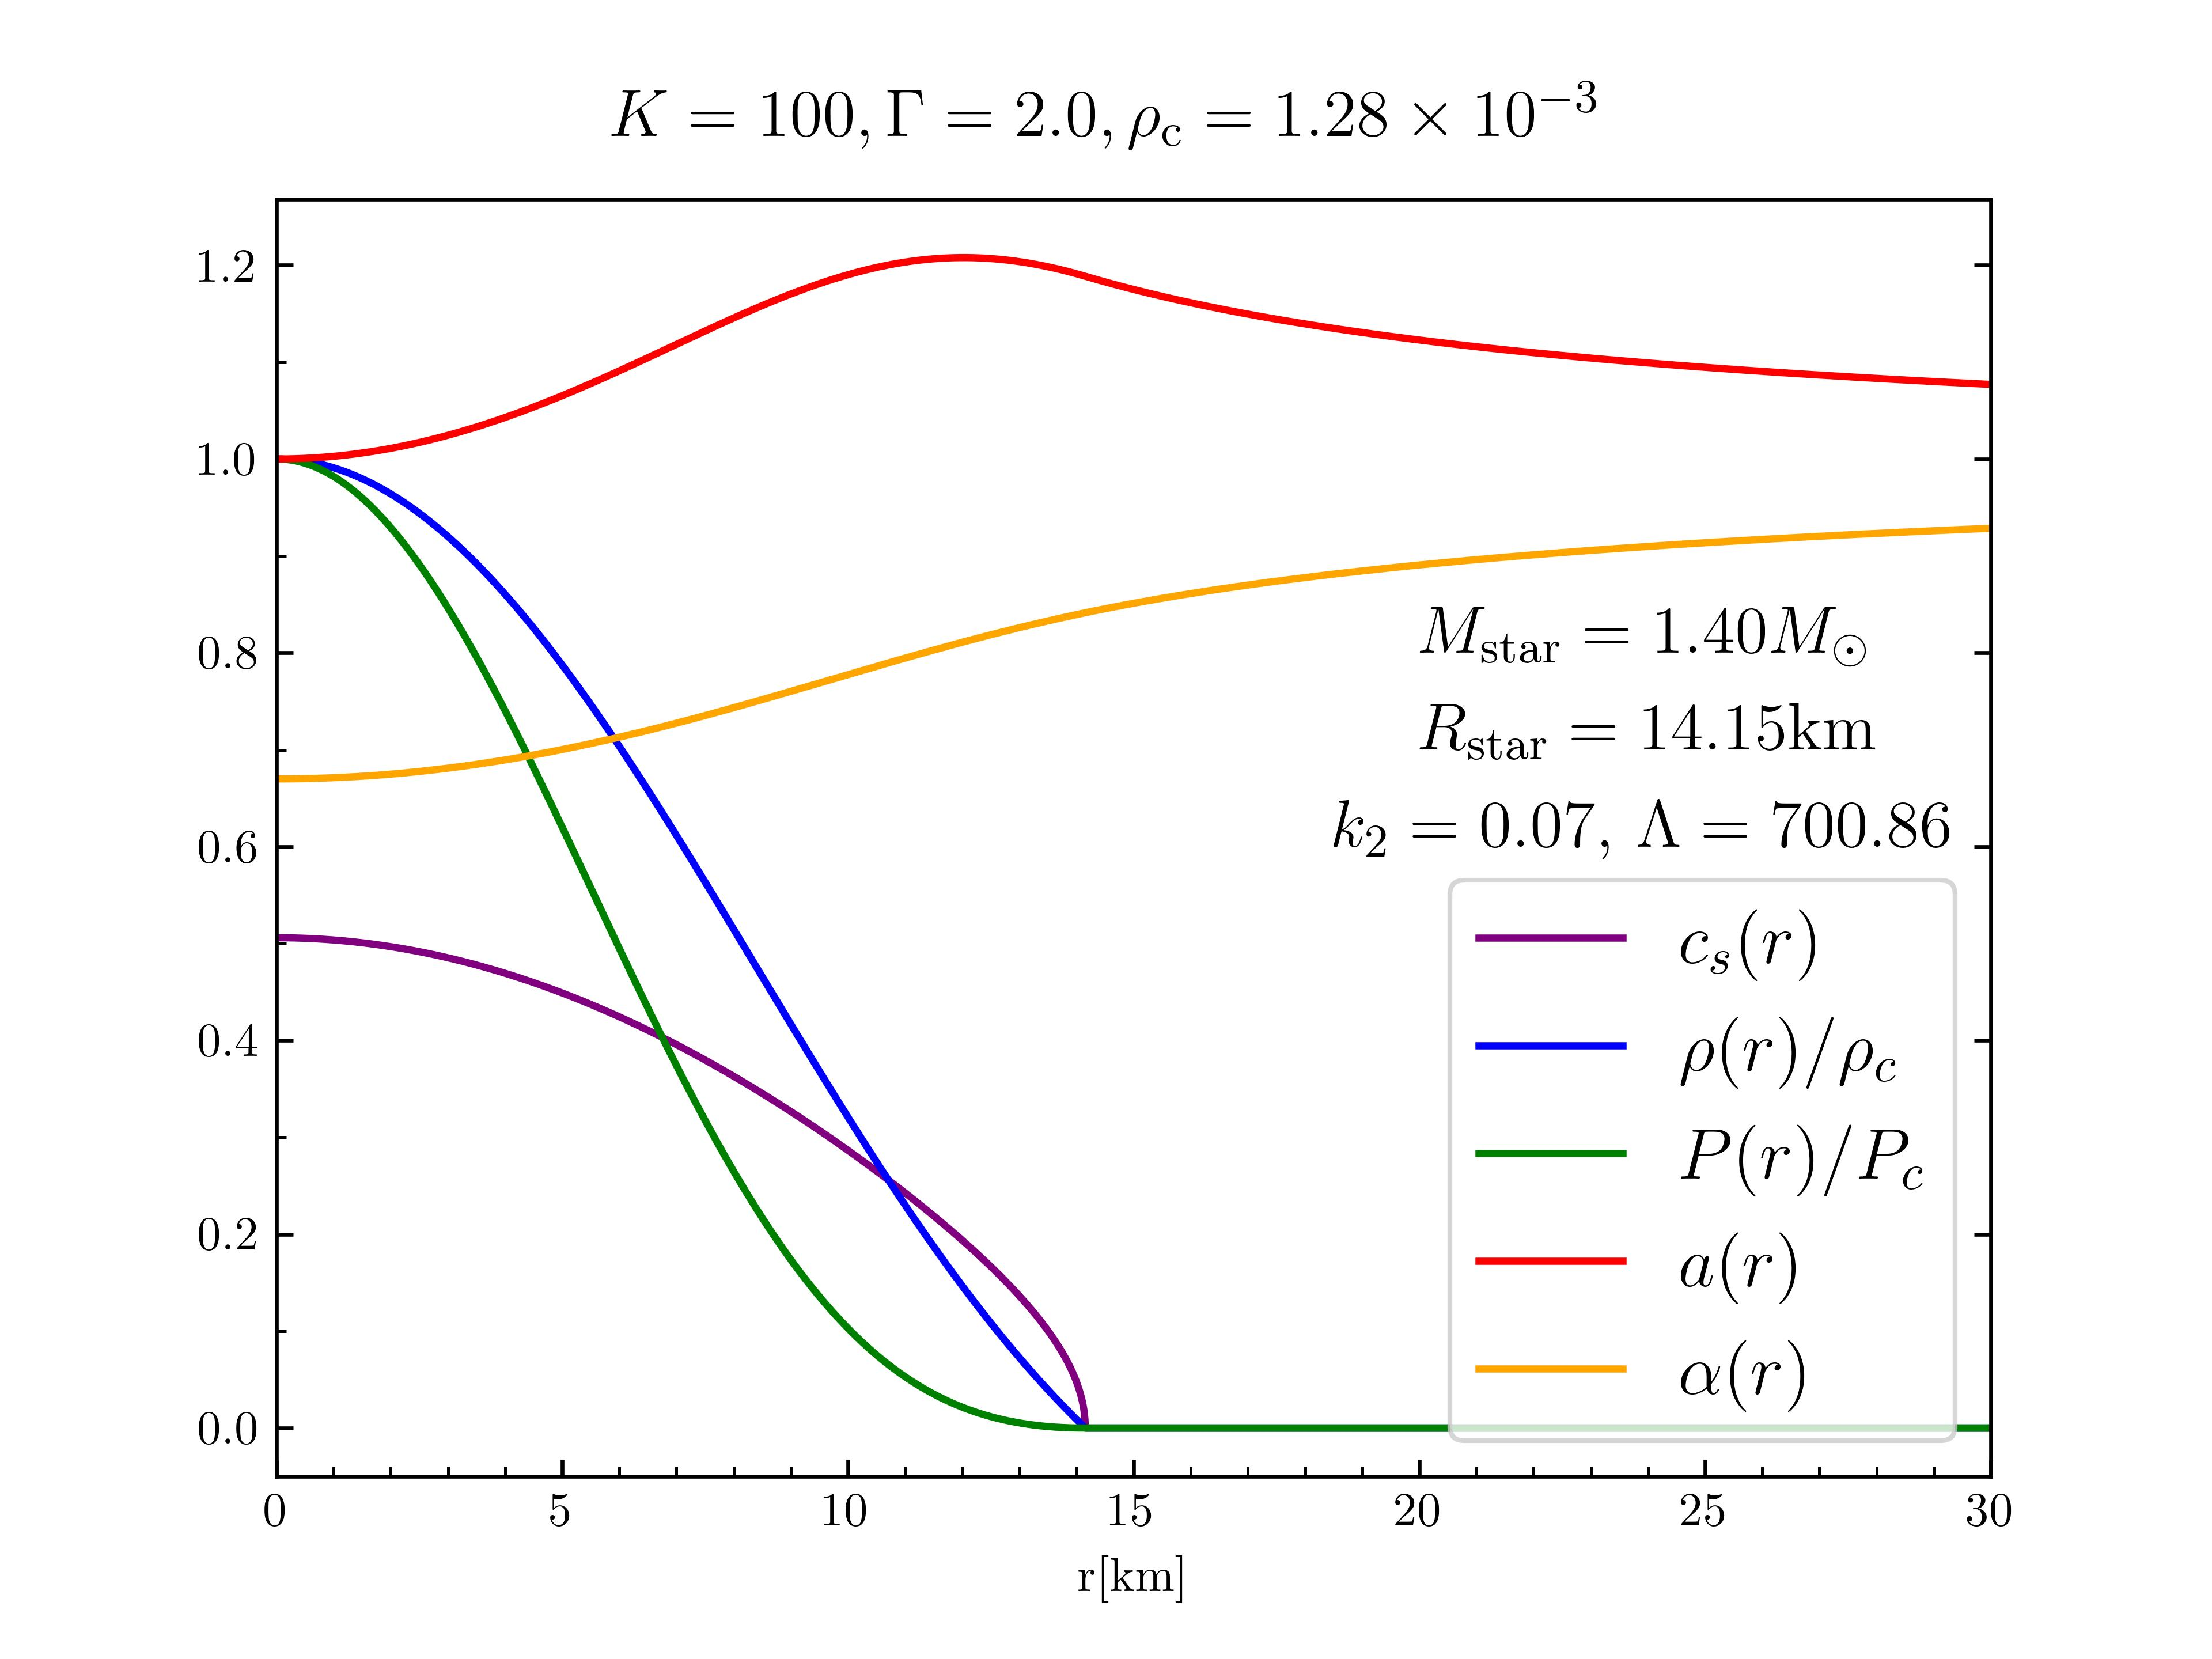
\includegraphics[scale=1]{tovRK4_OMAR}
		\caption{Integration of the TOV equations for a polytropic EoS such that $K=100.0$, $\Gamma=2.0$ and $\rho_c=1.28\times10^{-3}$ in code units.}
	\end{figure}
	%
	\appendix
	%
	\chapter{Christoffel Symbols for a Spherically Symmetric, Static, and Stationary Spacetime}
	%
	Let us consider the spacetime for a distribution with spherical symmetry that is also static and therefore, stationary. Then, its line element can be written as:
	%
	\begin{equation}
		ds^2 = -\alpha^2(r) dt^2 + X^2(r) dr^2 + r^2 d\theta^2 + r^2 \sin^2\theta\, d\phi^2
	\end{equation}
	%
	This metric is diagonal, since its associated matrix is:
	\begin{equation}
		g_{\mu\nu} = 
		\begin{pmatrix}
			-\alpha^2 & 0 & 0 & 0 \\
			0 & X^2 & 0 & 0 \\
			0 & 0 & r^2 & 0 \\
			0 & 0 & 0 & r^2 \sin^2\theta
		\end{pmatrix}
	\end{equation}
	%
	\section{Useful Relations for the Christoffel Symbols in a Diagonal Metric}
	%
	The following relations are taken from \cite{2004sgig.book.....C} and will be demonstrated below.\\
	
	If we take a metric $g_{\mu\nu}$ whose components can be written in diagonal form, such that $g_{\alpha\beta} = 0$ whenever $\alpha \neq \beta$, then:
	%
	\begin{align}
		\Gamma^{\lambda}_{\mu\nu} &= 0 \qquad \text{if }\mu,\nu,\lambda\text{ are all distinct.}\\
		\Gamma^{\lambda}_{\mu\mu} &= -\frac{1}{2}g^{\lambda\lambda}\partial_{\lambda}g_{\mu\mu} \\
		\Gamma^{\lambda}_{\mu\lambda} &= \partial_{\mu}(\ln\sqrt{|g_{\lambda\lambda}|}) \\
		\Gamma^{\lambda}_{\lambda\lambda} &= \partial_{\lambda}(\ln\sqrt{|g_{\lambda\lambda}|})
	\end{align}
	%
	Starting from the general definition of the Christoffel symbols:
	
	\begin{equation}
		\Gamma^\lambda_{\mu\nu} = \frac{1}{2} g^{\lambda\delta}
		(\partial_\nu g_{\delta\mu} + \partial_\mu g_{\delta\nu} - \partial_\delta g_{\mu\nu})
	\end{equation}
	%
	Let us now prove the identities given by Carroll:
	
	\begin{enumerate}[(i)]
		
		\item $\Gamma^\lambda_{\mu\nu} = 0$ for $\lambda \neq \mu \neq \nu$ and a diagonal metric
		
		\begin{align}
			\Gamma^\lambda_{\mu\nu} &= \frac{1}{2} g^{\lambda\delta} (\partial_\nu g_{\delta\mu} + \partial_\mu g_{\delta\nu} - \partial_\lambda g_{\mu\nu}) \\
			&= \frac{1}{2} g^{\lambda\lambda} (\partial_\nu g_{\lambda\mu} + \partial_\mu g_{\lambda\nu} - \partial_\lambda g_{\mu\nu})
		\end{align}
		
		Since the indices of the metric components do not match:
		$\lambda \neq \mu$, $\lambda \neq \nu$, $\mu \neq \nu \Rightarrow$, all combinations vanish because there are no off-diagonal components.\\\\
		$\therefore \boxed{\Gamma^\lambda_{\mu\nu} = 0}$
		
		\item $\Gamma^\lambda_{\mu\mu} = -\frac{1}{2}(g_{\lambda\lambda})^{-1}\partial_\lambda g_{\mu\mu}$ for $\mu\neq\lambda$ and a diagonal metric. Let us see that:
		
		\begin{align*}
			\Gamma^\lambda_{\mu\mu} &= \frac{1}{2}g^{\lambda\delta}(\partial_\mu g_{\delta\mu} + \partial_\mu g_{\delta\mu} - \partial_\delta g_{\mu\mu}) \\
			&= \frac{1}{2} g^{\lambda\lambda} (\partial_\mu g_{\lambda\mu} + \partial_\mu g_{\lambda\mu} - \partial_\lambda g_{\mu\mu}) \\
			&= -\frac{1}{2} g^{\lambda\lambda} \partial_\lambda g_{\mu\mu} = -\frac{1}{2} (g_{\lambda\lambda})^{-1} \partial_\lambda g_{\mu\mu} 
		\end{align*}
		%
		since $g^{\lambda\beta} = [g_{\lambda\beta}]^{-1}$ and $g_{\lambda\rho} g_\beta^\lambda = \delta_\lambda^\lambda$.
		
		$\therefore \boxed{\Gamma_{\mu\mu}^\lambda = -\frac{1}{2} g^{\lambda\lambda} \partial_\lambda g_{\mu\mu}}$
		
		\item $\Gamma_{\mu\lambda}^\lambda = \partial_\mu(\ln\sqrt{|g_{\lambda\lambda}|})$ \quad for $\mu\neq\lambda$ and a diagonal metric. Indeed:
		
		
		\begin{align*}
			\Rightarrow \Gamma_{\mu\lambda}^\lambda &= \frac{1}{2} g^{\lambda\delta} (\partial_\lambda g_{\delta\mu} + \partial_\mu g_{\delta\lambda} - \partial_\delta g_{\mu\lambda}) 
			= \frac{1}{2} g^{\lambda\lambda} (\partial_\lambda g_{\lambda\mu} + \partial_\mu g_{\lambda\lambda} - \partial_\lambda g_{\mu\lambda}) \\
			&= \frac{1}{2} g^{\lambda\lambda} \partial_\mu g_{\lambda\lambda} = \frac{1}{2} (g_{\lambda\lambda})^{-1} \partial_\mu g_{\lambda\lambda}
			= \frac{1}{2} \partial_\mu \ln |g_{\lambda\lambda}| \quad \text{because } g_{\lambda\lambda} <0 \text { o } g_{\lambda\lambda}>0 \\
			&= \partial_\mu \ln \sqrt{|g_{\lambda\lambda}|}.
		\end{align*}
		
		
		$\therefore \boxed{\Gamma_{\mu\lambda}^\lambda = \partial_\mu \ln\sqrt{|g_{\lambda\lambda}|}}$
		
		\item $\Gamma_{\lambda\lambda}^\lambda = \partial_\lambda(\ln\sqrt{|g_{\lambda\lambda}|})$ \quad for any diagonal metric:
		
		\begin{align*}
			\text{Ibidem,} \quad \Gamma_{\lambda\lambda}^\lambda &= \frac{1}{2} g^{\lambda\delta} (\partial_\lambda g_{\delta\lambda} + \partial_\lambda g_{\delta\lambda} - \partial_\delta g_{\lambda\lambda}) \\
			&= \frac{1}{2} g^{\lambda\lambda} (\partial_\lambda g_{\lambda\lambda} + \partial_\lambda g_{\lambda\lambda} - \partial_\lambda g_{\lambda\lambda}) = \frac{1}{2} (g_{\lambda\lambda})^{-1} \partial_\lambda g_{\lambda\lambda} \\
			&= \partial_\lambda \ln \sqrt{|g_{\lambda\lambda}|}.
		\end{align*}
		
		
		$\therefore \boxed{\Gamma_{\lambda\lambda}^\lambda = \partial_\lambda \ln\sqrt{|g_{\lambda\lambda}|}}$
		
		
		%
		\item $\Gamma_{\mu\lambda}^\lambda = \partial_\mu(\ln\sqrt{|g_{\lambda\lambda}|})$ \quad for $\mu\neq\lambda$ and a diagonal metric. Indeed:
		
		
		\begin{align*}
			\Gamma^\lambda_{\mu\lambda} 
			&= \frac{1}{2} g^{\lambda\delta} (\partial_\mu g_{\delta\lambda} + \partial_\lambda g_{\delta\mu} - \partial_\delta g_{\mu\lambda}) \\
			&= \frac{1}{2} g^{\lambda\lambda} (\partial_\mu g_{\lambda\lambda}) 
		\end{align*}
		
		because $g_{\delta\lambda}=0$ for $\delta\neq\lambda$ and $g_{\mu\lambda}=0$ for $\mu\neq\lambda$. Then:
		
		\begin{equation}
			\Gamma^\lambda_{\mu\lambda} 
			= \frac{1}{2} g^{\lambda\lambda} \partial_\mu g_{\lambda\lambda}
			= \frac{1}{2} \frac{1}{g_{\lambda\lambda}} \partial_\mu g_{\lambda\lambda}
			= \partial_\mu(\ln\sqrt{|g_{\lambda\lambda}|})
		\end{equation}
		
		\begin{equation}
			\therefore \boxed{\Gamma^\lambda_{\mu\lambda} = \partial_\mu(\ln\sqrt{|g_{\lambda\lambda}|})}
		\end{equation}
		
		\item $\Gamma^{\lambda}_{\lambda\lambda} = \partial_{\lambda}(\ln\sqrt{|g_{\lambda\lambda}|})$
		
		This expression follows directly from setting $\mu = \lambda$ in the previous identity:
		
		\begin{equation}
			\Gamma^{\lambda}_{\lambda\lambda}
			= \frac{1}{2} g^{\lambda\lambda} \partial_{\lambda} g_{\lambda\lambda}
			= \partial_{\lambda}(\ln\sqrt{|g_{\lambda\lambda}|})
		\end{equation}
		
		\begin{equation}
			\therefore \boxed{\Gamma^{\lambda}_{\lambda\lambda} = \partial_{\lambda}(\ln\sqrt{|g_{\lambda\lambda}|})}
		\end{equation}
		
	\end{enumerate}
	
	\vspace{0.5cm}
	
	\section{Explicit Christoffel Symbols for the Spherically Symmetric Static Metric}
	
	For the line element:
	
	\begin{equation}
		ds^2 = -\alpha^2(r) dt^2 + X^2(r) dr^2 + r^2 d\theta^2 + r^2 \sin^2\theta\, d\phi^2,
	\end{equation}
	
	the non-vanishing Christoffel symbols are the following:
	
	\begin{align*}
		\Gamma^t_{tr} &= \frac{\alpha'(r)}{\alpha(r)}, 
		&\Gamma^r_{tt} &= \frac{\alpha(r)\alpha'(r)}{X^2(r)}, 
		&\Gamma^r_{rr} &= \frac{X'(r)}{X(r)}, \\
		\Gamma^r_{\theta\theta} &= -\frac{r}{X^2(r)}, 
		&\Gamma^r_{\phi\phi} &= -\frac{r\sin^2\theta}{X^2(r)}, 
		&\Gamma^\theta_{r\theta} &= \Gamma^\phi_{r\phi} = \frac{1}{r}, \\
		\Gamma^\theta_{\phi\phi} &= -\sin\theta\cos\theta, 
		&\Gamma^\phi_{\theta\phi} &= \cot\theta.
	\end{align*}
	
	These can be verified directly using the general definition:
	
	\begin{equation}
		\Gamma^\lambda_{\mu\nu} = \frac{1}{2} g^{\lambda\sigma}
		\left( \partial_\mu g_{\sigma\nu} + \partial_\nu g_{\sigma\mu} - \partial_\sigma g_{\mu\nu} \right)
	\end{equation}
	
	and the inverse metric components:
	
	\begin{equation}
		g^{\mu\nu} = 
		\begin{pmatrix}
			-\alpha^{-2} & 0 & 0 & 0 \\
			0 & X^{-2} & 0 & 0 \\
			0 & 0 & r^{-2} & 0 \\
			0 & 0 & 0 & (r^2 \sin^2\theta)^{-1}
		\end{pmatrix}.
	\end{equation}
	
	A sufficient condition to define a static spacetime is to require that the components of the metric $g_{\mu\nu}$ do not depend on the coordinate time $t$ (it is stationary) and, moreover, that the metric satisfies $g_{\mu t} = 0$ if $\mu\neq t$.\\
	
	Let us then see that a metric of the form:
	
	\begin{equation}
		g_{\mu\nu} = {\rm diag}(-\alpha^2(r), X^2(r), r^2, r^2\sin^2\theta)
	\end{equation}
	%
	is static.\\
	
	Since the metric is static and spherically symmetric, the Christoffel symbols satisfy:
	
	\begin{equation}
		\Gamma^\lambda_{\mu\nu} = \Gamma^\lambda_{\nu\mu},
	\end{equation}
	and all components are independent of $t$ and $\phi$.  
	Therefore, the metric coefficients only depend on $r$, which implies:
	
	\begin{equation}
		\partial_t g_{\mu\nu} = \partial_\phi g_{\mu\nu} = 0.
	\end{equation}
	
	These simplifications are essential for deriving the Tolman–Oppenheimer–Volkoff (TOV) equations and for computing curvature tensors, such as the Ricci tensor, in spherically symmetric static spacetimes.\\
	
	Let us now compute explicitly the Christoffel symbols one by one. If we want to calculate the symbols that are independent from each other, there must be 40 in total taking into account that there are 10 symmetric combinations for the 2 lower indices:
	%
	\begin{equation}
		\begin{pmatrix}
			4+2-1 \\
			2 
		\end{pmatrix} = \begin{pmatrix}
			5 \\
			2 
		\end{pmatrix} = 10
	\end{equation}
	%
	and that there are 4 possible components to take for the free upper index.
	%
	\begin{enumerate}
		\item $\Gamma^t_{tt} = \partial_t(\ln\sqrt{|g_{tt}|}) = \partial_t(\ln\sqrt{\alpha^2}) = \partial_t\ln|\alpha(r)| = 0$
		
		\item $\Gamma^t_{rr} = -\frac{1}{2}g^{tt}\partial_t g_{rr} = -\frac{1}{2}\frac{1}{\alpha^2}\partial_t(X^2(r)) = 0$
		
		\item $\Gamma^t_{rt} = \Gamma^t_{tr} = \partial_r(\ln\sqrt{|g_{tt}|}) = \partial_r(\ln|\alpha(r)|) = \frac{\alpha'(r)}{\alpha(r)}$
		
		\item $\Gamma^t_{r\theta} = \Gamma^t_{\theta r} = 0 \quad ; \quad \text{(using i)}$
		
		\item $\Gamma^t_{r\phi} = \Gamma^t_{\phi r} = 0\quad; \quad \text{(using i)}$
		
		\item $\Gamma^t_{\theta\theta} = 0 \quad ;\quad\text{(using ii)}$
		
		\item $\Gamma^t_{\phi\phi} = 0 \quad ;\quad \text{(using ii)}$
		
		\item $\Gamma^t_{\theta\phi} = \Gamma^t_{\phi\theta} = 0 \quad; \quad \text{(using i)}$
		
		\item $\Gamma^t_{t\theta} = \Gamma^t_{\theta t} = 0 \quad ; \quad \text{(using iii)}, \text{ because } \partial_\theta \to 0 \text{ for } g_{tt}$
		
		\item $\Gamma^t_{t\phi} = \Gamma^t_{\phi t} = 0 \quad ;\quad \text{(using iii)}, \text{ because }  \partial_\phi \to 0 \text{ for } g_{tt}$
		
		\item $\Gamma^r_{tt} = -\frac{1}{2}g^{rr}\partial_r g_{tt} = -\frac{1}{2}\frac{1}{X^2}\partial_r(-\alpha^2(r)) = +\frac{\alpha(r)\alpha'(r)}{X^2(r)}$
		
		\item $\Gamma^r_{rr} = \partial_r(\ln\sqrt{g_{rr}}) = \partial_r(\ln\sqrt{X^2}) = \partial_r\ln X(r) = \frac{X'(r)}{X(r)}$
		
		\item $\Gamma^r_{tr} = \Gamma^r_{rt} = \partial_t(\ln\sqrt{g_{rr}}) = \partial_t(\ln X(r)) = 0$
		
		\item $\Gamma^r_{t\theta} = \Gamma^r_{\theta t} = 0 \quad ; \quad \text{(using i)}$
		
		\item $\Gamma^r_{t\phi} = \Gamma^r_{\phi t} = 0 \quad ; \quad\text{(using i)}$
		
		\item $\Gamma^r_{r\theta} = \Gamma^r_{\theta r} = 0 \quad ; \quad \text{(using iii)}, \text{ because } \partial_\theta \to 0$
		
		\item $\Gamma^r_{r\phi} = \Gamma^r_{\phi r} = 0 \quad;\quad \text{(using iii)}, \text{ because } \partial_\phi \to 0$
		
		\item $\Gamma^r_{\theta\theta} = -\frac{1}{2}g^{rr}\partial_r g_{\theta\theta} = -\frac{1}{2}\frac{1}{X^2}\partial_r(r^2) = -\frac{r}{X(r)}$
		
		\item $\Gamma_{\phi\phi} = -\frac{1}{2} g^{rr} \partial_r g_{\phi\phi} = -\frac{1}{2} \frac{1}{X^2} \partial_r (r^2\sin^2\theta) = -\frac{r\sin^2\theta}{X^2(r)}$ 
		
		\item $\Gamma^r_{\phi\phi} = \Gamma^r_{\phi\theta} = 0\quad;\quad \text{(using ii and iii)}, \text{ because } \partial_\theta \to 0 \text{ and }\partial_\phi \to 0$ 
		
		\item  $\Gamma^{\theta}_{tt} = 0 \; ; \; \quad \text{using ii), since } \partial_r \to 0 \text{ for all components except } g_{\phi\phi}$ 
		
		\item $\Gamma^{\theta}_{rr} = 0 \; ; \; \quad \text{using ii), since } \partial_r \to 0 \text{ for all components except } g_{\phi\phi} $
		
		\item $\Gamma^{\theta}_{\theta\theta} = 0\; ; \; \quad \text{using ii), since } \partial_r \to 0 \text{ for all components except } g_{\phi\phi}$
		
		\item $\Gamma^{\theta}_{\phi\phi} = -\frac{1}{2} g^{\theta\theta} \partial_{\theta} g_{\phi\phi} = -\frac{1}{2} \frac{1}{r^2} \partial_{\theta} (r^2\sin^2\theta) = -\frac{2\sin\theta\cos\theta}{2} = -\sin\theta\cos\theta$ 
		
		\item $\Gamma^{\theta}_{t\theta} = \Gamma^{\theta}_{\theta t} = 0 \quad \text{using iii), since } \partial_t \to 0$ 
		
		\item $ \Gamma^{\theta}_{r\theta} = \Gamma^{\theta}_{\theta r} = \partial_r \ln(\sqrt{g_{\theta\theta}}) = \partial_r(\ln \sqrt{r^2}) = \partial_r(\ln r) = \frac{1}{r}$ 
		
		\item $\Gamma^{\theta}_{tr} = \Gamma^{\theta}_{rt} = 0 \quad ; \quad \text{using i)}$ 
		
		\item $\Gamma^{\theta}_{r\phi} = \Gamma^{\theta}_{\phi r}=0\quad;\quad \text{using i)}$
		
		\item $\Gamma^{\theta}_{t\phi} = \Gamma^{\theta}_{\phi t} = 0 \quad;\quad \text{using i)}$ 
		
		\item $\Gamma^{\theta}_{\theta\phi} = \Gamma^{\theta}_{\phi\theta} = 0 \quad \text{using iii), since } \partial_{\phi} \to 0$ 
		
		\item $\Gamma^{\phi}_{tt} = 0 \quad \text{using ii)} \text{ since } \partial_{\phi} \to 0$ 
		
		\item $\Gamma^{\phi}_{rr} = 0 \quad \text{using ii)} \text{ since } \partial_{\phi} \to 0$ 
		
		\item $\Gamma^{\phi}_{\theta\theta} = 0 \quad \text{using ii)} \text{ since } \partial_{\phi} \to 0$
		
		\item $\Gamma^{\phi}_{\phi\phi} = 0 \quad \text{using ii)} \text{ since } \partial_{\phi} \to 0$
		
		\item $\Gamma^{\phi}_{t\phi} = \Gamma^{\phi}_{\phi t} = 0 \quad \text{using iii), since } \partial_t g_{\phi\phi} = 0$ 
		
		\item $\Gamma^{\phi}_{r\phi} = \Gamma^{\phi}_{\phi r} = \partial_r \ln(\sqrt{g_{\phi\phi}}) = \partial_r \ln(r\sin\theta) = \frac{\sin\theta}{r\sin\theta} = \frac{1}{r}$ 
		
		\item $\Gamma^{\phi}_{\theta\phi} = \Gamma^{\phi}_{\phi\theta} = \partial_{\theta} \ln(\sqrt{g_{\phi\phi}}) = \partial_{\theta} \ln(r\sin\theta) = \frac{r\cos\theta}{r\sin\theta} = \cot\theta$ 
		
		\item $\Gamma^{\phi}_{tr} = \Gamma^{\phi}_{rt} = 0 \quad ; \quad\text{(using i)}$
		
		\item $\Gamma^{\phi}_{r\theta} = \Gamma^{\phi}_{\theta r} = 0 \quad ; \quad\text{(using i)} $
		
		\item $\Gamma^{\phi}_{t\theta} = \Gamma^{\phi}_{\theta t} = 0\quad ; \quad\text{(using i)}$
	\end{enumerate}
	%
	Let us see that these values agree with those calculated by Griselda Arroyo and Sean Carroll:
	%
	\begin{align*}
		\Gamma^t_{tt} &= 0 & \Gamma^r_{\theta\theta} &= -\frac{r}{X^2} \\
		\Gamma^t_{tr} = \Gamma^t_{rt} &= \frac{\alpha'}{\alpha} & \Gamma^r_{\phi\phi} &= -\frac{r\sin^2\theta}{X^2} \\
		\Gamma^t_{rr} &= 0 & \Gamma^\theta_{r\theta} = \Gamma^\theta_{\theta r} &= \frac{1}{r} \\
		\Gamma^r_{tt} &= \frac{\alpha\alpha'}{X^2} & \Gamma^\theta_{\phi\phi} &= -\sin\theta \cos\theta \\
		\Gamma^r_{tr} = \Gamma^r_{rt} &= 0 & \Gamma^\phi_{r\phi} = \Gamma^\phi_{\phi r} &= \frac{1}{r} \\
		\Gamma^r_{rr} &= \frac{X'}{X} & \Gamma^\phi_{\theta\phi} = \Gamma^\phi_{\phi\theta} &= \cot\theta
	\end{align*}
	%
	\chapter{Einstein equations for a spherically symmetric and static metric  }
	%
	With the calculations of Appendix A, we can now compute the components of the Ricci tensor $R_{\mu\nu}$ and the Einstein tensor $G_{\mu\nu}$:
	%
	\begin{equation}
		R_{\mu\nu} = \partial_\sigma\Gamma^\sigma_{\mu\nu} - \partial_\nu\Gamma^\sigma_{\mu\sigma} + \Gamma^\sigma_{\sigma\tau}\Gamma^\tau_{\mu\nu} - \Gamma^\sigma_{\nu\tau}\Gamma^\tau_{\mu\sigma}
	\end{equation}
	%
	\begin{equation}
		G_{\mu\nu} = R_{\mu\nu}- \dfrac{1}{2}Rg_{\mu\nu}
	\end{equation}
	%
	First, let us begin with the Ricci tensor. Performing the explicit component-by-component calculations:
	
	%
	\begin{align*}
		R_{tt} &= \partial_\sigma\Gamma^\sigma_{tt} - \partial_t\Gamma^\sigma_{t\sigma} + \Gamma^\sigma_{\sigma\tau}\Gamma^\tau_{tt} - \Gamma^\sigma_{t\tau}\Gamma^\tau_{t\sigma} \\
		&= \partial_t\Gamma^t_{tt} + \partial_r\Gamma^r_{tt} - \partial_t\Gamma^t_{tt} - \partial_t\Gamma^r_{tr} + \Gamma^t_{tt}\Gamma^t_{tt} - \Gamma^t_{tt}\Gamma^t_{tt} \\
		&\quad + \Gamma^r_{\sigma r}\Gamma^r_{tt} - \Gamma^r_{tt}\Gamma^t_{tr} + \Gamma^r_{\theta\theta}\Gamma^r_{tt} + \Gamma^\phi_{r\phi}\Gamma^r_{tt} \\
		&= \partial_r\Gamma^r_{tt} + \Gamma^r_{rr}\Gamma^r_{tt} - \Gamma^r_{tt}\Gamma^t_{tr} + \frac{1}{r}\frac{\alpha\alpha'}{X^2} + \frac{1}{r}\frac{\alpha\alpha'}{X^2} \\
		&= \partial_r\left(\frac{\alpha\alpha'}{X^2}\right) + \frac{X'}{X}\frac{\alpha\alpha'}{X^2} - \frac{\alpha\alpha'}{X^2}\frac{\alpha'}{\alpha} + \frac{2}{r}\frac{\alpha\alpha'}{X^2} \\
		&= \frac{(\alpha')^2}{X^2} + \frac{\alpha\alpha''}{X^2} - \frac{2\alpha\alpha'X'}{X^3} + \frac{\alpha\alpha'X'}{X^3} - \frac{(\alpha')^2}{X^2} + \frac{2}{r}\frac{\alpha\alpha'}{X^2}
	\end{align*}
	%
	\begin{equation}
		\therefore \boxed{R_{tt} = \frac{\alpha\alpha''}{X^2} - \frac{\alpha\alpha'X'}{X^3} + \frac{2}{r}\frac{\alpha\alpha'}{X^2}}
	\end{equation}
	%
	\begin{align*}
		R_{rr} &= \partial_\sigma\Gamma^{\sigma}_{rr} - \partial_r\Gamma^{\sigma}_{r\sigma} + \Gamma^{\sigma}_{\epsilon\sigma}\Gamma^{\epsilon}_{rr} - \Gamma^{\sigma}_{\epsilon r}\Gamma^{\epsilon}_{r\sigma}\\
		&= \partial_r\Gamma^r_{rr} - \partial_r\Gamma^t_{rt} - \partial_r\Gamma^r_{rr} + \Gamma^t_{rt}\Gamma^r_{rr} + \Gamma^{\theta}_{r\theta}\Gamma^r_{rr} + \Gamma^{\phi}_{r\phi}\Gamma^r_{rr} - \Gamma^t_{tr}\Gamma^t_{rt} \\
		& = -\partial_r\left(\frac{\alpha'}{\alpha}\right) + \Gamma^t_{rt}\left(\Gamma^r_{rr} - \Gamma^t_{rt}\right) + \Gamma^{\theta}_{r\theta}\Gamma^r_{rr} + \Gamma^{\phi}_{r\phi}\Gamma^r_{rr} \\
		& = -\frac{\alpha''}{\alpha} + \frac{(\alpha')^2}{\alpha^2} + \frac{\alpha'X'}{\alpha X} - \frac{(\alpha')^2}{\alpha^2} + \frac{1}{r}\frac{X'}{X} + \frac{1}{r}\frac{X'}{X} \\
		&= \frac{\alpha'X'}{\alpha X} - \frac{\alpha''}{\alpha} + \frac{2}{r}\frac{X'}{X}  
	\end{align*}
	%
	\begin{equation}
		\therefore \boxed{R_{rr}=\frac{\alpha'X'}{\alpha X} - \frac{\alpha''}{\alpha} + \frac{2}{r}\frac{X'}{X} }
	\end{equation}
	%
	\begin{align*}
		R_{\theta\theta} &= \partial_\sigma\Gamma^{\sigma}_{\theta\theta} - \partial_\theta\Gamma^{\sigma}_{\theta\sigma} + \Gamma^{\sigma}_{\epsilon\sigma}\Gamma^{\epsilon}_{\theta\theta} - \Gamma^{\sigma}_{\epsilon\theta}\Gamma^{\epsilon}_{\theta\sigma}\\
		&= \partial_r\Gamma^r_{\theta\theta} - \partial_\theta\Gamma^{\phi}_{\theta\phi} + \Gamma^{\sigma}_{r\sigma}\Gamma^r_{\theta\theta} - \Gamma^{\sigma}_{r\theta}\Gamma^{r}_{{\theta\sigma}} - \Gamma^{\sigma}_{\theta\theta}\Gamma^{\theta}_{\theta\sigma} - \Gamma^{\sigma}_{\phi\theta}\Gamma^{\phi}_{\theta\sigma} \\
		& = \partial_r\left(-\frac{r}{X^2}\right) - \partial_\theta(\cot\theta) + \left(\Gamma^t_{rt} + \Gamma^r_{rr} + \Gamma^{\theta}_{\theta} + \Gamma^{\phi}_{\phi}\right)\Gamma^r_{\theta\theta}
		-\Gamma^{\theta}_{r\theta}\Gamma^{r}_{\theta\theta} - \Gamma^{r}_{\theta\theta}\Gamma^{\theta}_{\theta r} - \Gamma^{\phi}_{\theta\theta}\Gamma^{\phi}_{\phi\phi} \\
		&= -\frac{1}{X^2} + \frac{2rX'}{X^3} + \csc^2\theta - \left(\frac{\alpha'}{\alpha}+\frac{X'}{X}+\frac{2}{r}\right)r\frac{2}{X^2} + \frac{2}{r}\cdot\frac{r}{X^2} 
		-\cot^2\theta \\
		&= -\frac{1}{X^2} + \frac{rX'}{X^3} + 1 - \frac{r\alpha'}{X^2\alpha} 
	\end{align*}
	%
	\begin{equation}
		\therefore \boxed{R_{\theta\theta}== \frac{1}{X^2}\left(\frac{rX'}{X} - \frac{r\alpha'}{\alpha} - 1\right) + 1}
	\end{equation}
	%
	\begin{align*}
		R_{\phi\phi} &= \partial_{\sigma}\Gamma^{\sigma}_{\phi\phi} - \partial_{\phi}\Gamma^{\sigma}_{\phi\sigma} + \Gamma^{\sigma}_{\epsilon\sigma}\Gamma^{\epsilon}_{\phi\phi} - \Gamma^{\sigma}_{\epsilon\phi}\Gamma^{\epsilon}_{\phi\sigma} \\
		&= \partial_r\Gamma^r_{\phi\phi} + \partial_{\theta}\Gamma^{\theta}_{\phi\phi} + \Gamma^t_{\epsilon t}\Gamma^{\epsilon}_{\phi\phi} + \Gamma^r_{\epsilon r}\Gamma^{\epsilon}_{\phi\phi} + \Gamma^{\theta}_{\epsilon\theta}\Gamma^{\epsilon}_{\phi\phi} + \Gamma^{\phi}_{\epsilon\phi}\Gamma^{\epsilon}_{\phi\phi} \\
		&\quad - \Gamma^r_{\epsilon\phi}\Gamma^{\epsilon}_{\phi r} - \Gamma^{\theta}_{\epsilon\phi}\Gamma^{\epsilon}_{\phi\theta} - \Gamma^{\phi}_{\epsilon\phi}\Gamma^{\epsilon}_{\phi\phi} \\
		&= \partial_r\Gamma^r_{\phi\phi} + \partial_{\theta}\Gamma^{\theta}_{\phi\phi} + \Gamma^t_{rt}\Gamma^r_{\phi\phi} + \Gamma^r_{rr}\Gamma^r_{\phi\phi} + \Gamma^{\theta}_{r\theta}\Gamma^r_{\phi\phi} + \Gamma^{\phi}_{r\phi}\Gamma^r_{\phi\phi} + \Gamma^{\phi}_{\theta\phi}\Gamma^{\theta}_{\phi\phi} \\
		&\quad - \Gamma^r_{\phi\phi}\Gamma^{\phi}_{\phi r} - \Gamma^{\theta}_{\phi\phi}\Gamma^{\phi}_{\theta\theta} - \Gamma^{\phi}_{r\phi}\Gamma^r_{\phi\phi} - \Gamma^{\phi}_{\theta\phi}\Gamma^{\theta}_{\phi\phi} - \Gamma^{\phi}_{\phi\phi}\Gamma^{\theta}_{\phi\phi} \\
		&= -\frac{\sin^2\theta}{X^2} + \frac{r\sin^2\theta X'}{X^3} - \cos^2\theta + \sin^2\theta + \cos^2\theta - \frac{r\sin^2\theta\alpha'}{X^2} \\
		&= \frac{r\sin^2\theta X'}{X^3} - \frac{r\sin^2\theta \alpha'}{\alpha X^2} - \frac{\sin^2\theta}{X^2} + \sin^2\theta
	\end{align*}
	%
	\begin{equation}
		\therefore \boxed{R_{\phi\phi} = \frac{1}{X^2}\sin^2\theta\left[r\frac{X'}{X} - r\frac{\alpha'}{\alpha} - 1\right] + \sin^2\theta = \sin^2\theta R_{\theta\theta}}
	\end{equation}
	%
	\newpage
	Then, we can arrive to an expression for the Ricci curvature scalar:
	
	\begin{align*}
		R &= g^{tt}R_{tt} + g^{rr}R_{rr} + g^{\theta\theta}R_{\theta\theta} + g^{\phi\phi}R_{\phi\phi}\\
		&
		= -\frac{1}{\alpha^2}R_{tt} + \frac{1}{X^2}R_{rr} + \frac{1}{r^2}R_{\theta\theta} + \frac{1}{r^2\sin^2\theta}\sin^2\theta R_{\theta\theta} \\
		&= -\frac{\alpha''}{\alpha X^2} + \frac{\alpha'X'}{\alpha X^3} - \frac{2\alpha'}{r\alpha X^2} + \frac{\alpha'X'}{\alpha X^3} - \frac{\alpha''}{\alpha X^2}\\
		&
		+ \frac{2}{r}\frac{X'}{X^3} + \frac{2X'}{rX^3} - \frac{2\alpha'}{r\alpha X^2} - \frac{2}{r^2X^2} + \frac{2}{r^2} \\
		&= -\frac{2\alpha''}{\alpha X^2} + \frac{2\alpha'X'}{\alpha X^3} - \frac{4\alpha'}{r\alpha X^2} + \frac{4X'}{rX^3} - \frac{2}{r^2X^2} + \frac{2}{r^2}
	\end{align*}
	%
	\begin{equation}
		\therefore \boxed{R= -\frac{2}{X^2}\left[\frac{\alpha''}{\alpha} - \frac{\alpha'X'}{\alpha X} + \frac{2}{r}\left(\frac{\alpha'}{\alpha} - \frac{X'}{X}\right) + \frac{1}{r^2}(1-X^2)\right]}\\
	\end{equation}
	%
	Now, it's time to write down the full Einstein equations component by component:
	%%%
	\begin{equation}
		G_{\mu\nu} = 8\pi T_{\mu\nu},
	\end{equation}
	%
	
	Let's study one by one the non-vanishing terms and components of these equations, that are obtained for our spacetime and our matter-energy background:
	%%%
	\begin{enumerate}
		\item $G_{tt} = 8\pi T_{tt}$
		\begin{align*}
			G_{tt} &= R_{tt}-\frac{1}{2}g_{tt}(g^{tt}R_{tt} + g^{rr}R_{rr} + g^{\theta\theta}R_{\theta\theta} + g^{\phi\phi}R_{\phi\phi})\\
			&= \frac{R_{tt}}{2} + \frac{1}{2}\alpha^2(g^{rr}R_{rr} + g^{\theta\theta}R_{\theta\theta} + g^{\phi\phi}R_{\phi\phi})\\
			\Rightarrow G_{tt}&= \frac{\alpha\alpha''}{2X^2} - \frac{\alpha\alpha'X'}{2X^3} + \frac{\alpha\alpha'}{rX^2} + \frac{\alpha\alpha'X'}{2X^3} - \frac{\alpha\alpha''}{2X^2} + \frac{2\alpha^2X'}{rX^3} - \frac{\alpha\alpha'}{rX^2} - \frac{\alpha^2}{r^2X^2} + \frac{\alpha^2}{r^2}
		\end{align*}
		%
		\begin{equation}
			\therefore \boxed{ G_{tt} = \frac{\alpha^2}{r^2X^3}(2rX' + X^3 - X)}\\
		\end{equation}
		%
		For the energy-momentum tensor of a perfect fluid, we have:
		%
		\begin{equation}
			T_{\mu\nu} = \rho h u^\mu u^\nu + Pg^{\mu\nu} 
		\end{equation}
		%
		Computing the $tt$ component, we have:
		\begin{equation}
			T_{tt} = \rho h(u_t)^2 - P\alpha^2
		\end{equation}
		%
		If we consider the 4-velocity of a fluid element as the time-like tangent vector from the worldline of an Eulerian observer respect to it, then we get:
		\begin{equation}
			u_\mu = n_\mu = (\alpha, 0, 0, 0)
		\end{equation}
		
		\begin{equation}
			T_{tt} = \rho h \alpha^2 - P\alpha^2 = \alpha^2(\rho h - P)
		\end{equation}
		%
		Therefore,
		%
		\begin{align}
			G_{tt} &= 8\pi T_{tt}\\
			& \frac{\alpha^2}{r^2X^3}(2rX' + X^3 - X) = 8\pi\alpha^2(\rho h - P) \\
			& \frac{1}{r^2}\frac{1}{X^2}\left(2r\frac{X'}{X} - 1 + X^2\right) = 8\pi(\rho h - P)
		\end{align}
		%
		Next, we shall consider the following transformation of variables:
		%
		\begin{equation}
			m(r) = \frac{r}{2}\left(1 - \frac{1}{X^2}\right)
		\end{equation}
		%
		which equivalently is,
		%
		\begin{equation}
			X^2 = \left(1 - \frac{2m(r)}{r}\right)^{-1}
		\end{equation}
		%
		Let be $f = \ln X^2 \Rightarrow 2\ln X = -\ln\left(1 - \frac{2m(r)}{r}\right)$
		\begin{align*}
			2\frac{X'}{X} &= -\left(\frac{-2m'(r)}{r} + \frac{2m(r)}{r^2}\right)\frac{1}{1 - \frac{2m(r)}{r}}\\
			\frac{X'}{X} &= \left(\frac{m'(r)}{r} - \frac{m(r)}{r^2}\right)\frac{1}{1 - \frac{2m(r)}{r}}
		\end{align*}
		%
		Returning to Einstein's equations in their $tt$ component:%
		\begin{align*}
			\Rightarrow &\;\frac{1}{r^2}\left(1-\frac{2m(r)}{r}\right)\left(\frac{2m'(r)-\frac{2m(r)}{r}}{1-\frac{2m(r)}{r}}-1+\frac{1}{1-\frac{2m(r)}{r}}\right)\\
			&= \frac{1}{r^2}\left(1-\frac{2m(r)}{r}\right)\left(\frac{2m'(r)-\frac{2m(r)}{r}-1+\frac{2m(r)}{r}+1}{1-\frac{2m(r)}{r}}\right)\\
			&= \frac{1}{r^2}\;(2m'(r)) \\
			&= 8\pi[\rho h-P] = 8\pi\left[\rho(1+\epsilon)\frac{P}{\rho}-P\right]\\
			&= 8\pi[\rho(1+\epsilon_{int})+P-P] = 8\pi\rho(1+\epsilon)\\
			&= 8\pi e.
		\end{align*}
		
		\begin{equation*}
			\therefore \boxed{m'(r)=\frac{dm}{dr}=4\pi r^2e}
		\end{equation*}
		
		\item $G_{rr}=8\pi T_{rr}$
		
		Analogously, 
		%
		\begin{align*}
			G_{rr}&=R_{rr}-\frac{1}{2}X^2(g^{tt}R_{tt}+g^{\theta\theta}R_{\theta\theta}+g^{\phi\phi}R_{\phi\phi})\\
			G_{rr} &= \frac{\alpha'X'}{2\alpha X}-\frac{\alpha''}{2\alpha}+\frac{X'}{rX}+\frac{\alpha''}{2\alpha}-\frac{\alpha'X'}{2\alpha X}+\frac{\alpha'}{r\alpha}
			-\frac{X'}{rX}+\frac{\alpha'}{r\alpha}+\frac{1}{r^2}-\frac{X^2}{r^2}
		\end{align*}
		
		\begin{equation*}
			\therefore \boxed{G_{rr}=\frac{2\alpha'}{r\alpha}+\frac{1-X^2}{r^2}}
		\end{equation*}
		
		\begin{align*}
			&\Rightarrow G_{rr} = 8\pi T_{rr} \\
			&\frac{2\alpha'}{\alpha r} + \frac{1}{r^2} - \frac{1}{r^2\left(1-\frac{2m(r)}{r}\right)} = 8\pi P\left(1-\frac{2m(r)}{r}\right) \\
			&\Rightarrow\frac{\alpha'}{\alpha} = \frac{4\pi P r}{1-\frac{2m(r)}{r}} + \frac{1}{2r}\;\frac{1}{1-\frac{2m(r)}{r}} - \frac{1}{2r} \\
			&= \frac{1}{1-\frac{2m(r)}{r}}\left[4\pi P r + \frac{1}{2r}\;\left(1-\left(1-\frac{2m(r)}{r}\right)\right)\right] \\
			&= \frac{1}{1-\frac{2m(r)}{r}}\left(4\pi Pr + \frac{m(r)}{r^2}\right)
		\end{align*}
		%
		\begin{equation}
			\therefore \boxed{\Rightarrow \frac{\alpha'}{\alpha}= \frac{1}{\alpha}\frac{d\alpha}{dr}=\frac{m(r) + 4\pi P r^3}{r^2\left(1-\frac{2m(r)}{r}\right)}}
		\end{equation}
		%
		\item Finally, for the last equation, we will use the conservation of the energy-momentum tensor:
		%
		\begin{equation}
			\nabla_\mu T^{\mu\nu} = 0
		\end{equation}
		%
		Starting from the standard definition of the divergence for a 2-rank tensor:%
		\begin{equation}
			\nabla_\mu T^{\mu\nu} = \partial_\mu T^{\mu\nu} + \Gamma^\mu_{\mu\lambda}T^{\lambda\nu} + \Gamma^\nu_{\mu\lambda}T^{\mu\lambda} = 0    
		\end{equation}
		%
		Expanding the terms for the component $\nu = r$:
		%
		\begin{align*}
			\Rightarrow \nabla_\mu T^{\mu r} &= \partial_r T^{rr} + \Gamma^\mu_{\mu r}T^{rr} + \Gamma^r_{\mu\lambda}T^{\mu\lambda}\\
			&= \partial_r T^{rr} + \left(\Gamma^t_{tr} + \Gamma^r_{rr} + \Gamma^\theta_{r} + \Gamma^\phi_r\right)T^{rr}+ \Gamma^r_{tt}T^{tt} + \Gamma^r_{rr}T^{rr} + \Gamma^r_{\theta\theta}T^{\theta\theta} + \Gamma^r_{\phi\phi}T^{\phi\phi}\\
			&= 0
		\end{align*}
		%
		Now, it is appropriate to express the components of the energy-momentum tensor with upper indices (contravariant) and write the Christoffel symbols that we need for the calculation:
		\begin{align*}
			T^{tt} &= \rho h\left(u^t\right)^2 + pg^{tt} = \frac{1}{\alpha^2}(\rho h - P) = \frac{1}{\alpha^2}e & \Gamma^t_{tr} &= \frac{\alpha'}{\alpha} & \Gamma^r_{tt} &= \frac{\alpha\alpha'}{X^2} \\
			T^{rr} &= \frac{P}{X^2} & \Gamma^r_{rr} &= \frac{X'}{X} & \Gamma^r_{\theta\theta} &= -\frac{r}{X^2} \\
			T^{\theta\theta} &= \frac{P}{r^2} & \Gamma^\theta_{\theta r} &= \frac{1}{r} & \Gamma^r_{\phi\phi} &= -\frac{r\sin^2\theta}{X^2} \\
			T^{\phi\phi} &= \frac{P}{r^2\sin^2\theta} & \Gamma^\phi_{\phi r} &= \frac{1}{r}
		\end{align*}
		%
		Then,
		%
		\begin{align*}
			\Rightarrow \nabla_\mu T^{\mu r} &= \partial_r\left(\frac{P}{X^2}\right) + \left(\frac{\alpha'}{\alpha} + \frac{X'}{X} + \frac{2}{r}\right)\frac{P}{X^2} + \frac{\alpha'}{\alpha X^2}e + \frac{X'}{X^3}P - \frac{2P}{rX^2} \\
			&= \frac{P'}{X^2} - \frac{2PX'}{X^3} + \frac{\alpha'P}{\alpha X^2} + \frac{2PX'}{X^3} + \frac{2P}{rX^2} + \frac{\alpha'}{\alpha X^2}e - \frac{2P}{rX^2} \\
			&= \frac{P'}{X^2} + \frac{\alpha'}{\alpha X^2}(e+P) = 0 \\
			\Rightarrow P' &= -\frac{\alpha'}{\alpha}(e + P)
		\end{align*}
		%
		So finally, we can find that:
		%
		\begin{equation*}
			\therefore \boxed{\frac{dP}{dr} = -(e+P)\frac{1}{\alpha}\frac{d\alpha}{dr} = -(e+P)\frac{m + 4\pi Pr^3}{r^2\left(1-\frac{2m}{r}\right)}}
		\end{equation*}
	\end{enumerate}
	%
	
	%
	\bibliographystyle{aasjournal}
	\bibliography{refs.bib}
	\nocite{*}
	%
	
\end{document}
